% Annals of Applied Statistics submission (IMS imsart class).
% imsart.cls / imsart.sty / spr-ims-nameyear.bst are included (VTeX texsupport.ims-aoas,
% MIT licence, see LICENSE-imsart);
% the IMS class is used. Otherwise the document falls back to the article class
% with minimal stand-ins for the imsart front-matter macros, so it always compiles.
\IfFileExists{imsart.cls}{%
  \documentclass[aoas,preprint]{imsart}\def\IMSfallback{0}%
}{%
  \documentclass[11pt]{article}\def\IMSfallback{1}%
}

\makeatletter
\ifnum\IMSfallback=1
  \usepackage[margin=1in]{geometry}
  \newcommand{\startlocaldefs}{}
  %\newcommand{\endlocaldefs}{}
  \newenvironment{frontmatter}{}{}
  \newcommand{\runtitle}[1]{}
  \def\IMS@authors{}
  \renewcommand{\author}[2][]{%
    \ifx\IMS@authors\@empty\g@addto@macro\IMS@authors{#2}%
    \else\g@addto@macro\IMS@authors{\and #2}\fi
    \gdef\@author{\IMS@authors}}
  \newcommand{\fnms}[1]{#1}
  \newcommand{\snm}[1]{#1}
  \newcommand{\ead}[2][]{}
  \newcommand{\printead}[2][]{}
  \newcommand{\address}[2][]{}
  % the aug block ends the title block: typeset the title after it
  \newenvironment{aug}{\let\and\relax}{\aftergroup\maketitle}
  \newenvironment{keyword}{\par\noindent\textbf{Keywords:} \ignorespaces}{\par}
  \newcommand{\kwd}[1]{#1;\ }
  \newenvironment{funding}{\section*{Funding}}{}
  \newenvironment{acks}[1][Acknowledgments]{\section*{#1}}{}
  \newenvironment{supplement}{\section*{Supplementary material}}{}
  \newcommand{\stitle}[1]{\textbf{#1.}\ }
  \newcommand{\sdescription}[1]{#1}
\fi
\makeatother

\RequirePackage{amsthm,amsmath,amsfonts,amssymb}
\RequirePackage[authoryear]{natbib}
\RequirePackage[colorlinks,citecolor=blue,urlcolor=blue]{hyperref}
\RequirePackage{graphicx}
\RequirePackage{booktabs}
\RequirePackage{multirow}
\RequirePackage{bm}
\RequirePackage{xcolor}
\makeatletter
% Labels of the other document (main <-> supplement), read from a file of its \newlabel
% lines (made by build.sh); the IMS class does not allow the xr package.
\def\extlabels@nl#1#2{\@ifundefined{r@#1}{\global\@namedef{r@#1}{#2}}{}}
\def\extlabels#1{\IfFileExists{#1}{\begingroup\let\newlabel\extlabels@nl
  \input{#1}\endgroup}{}}
\makeatother
\AtBeginDocument{\extlabels{supp-labels.tex}}

\startlocaldefs
\numberwithin{equation}{section}
\theoremstyle{plain}
\newtheorem{proposition}{Proposition}
\theoremstyle{definition}
\newtheorem{remark}{Remark}
% notation
\newcommand{\bx}{\bm{x}}
\newcommand{\bz}{\bm{z}}
\newcommand{\bw}{\bm{w}}
\newcommand{\bv}{\bm{v}}
\newcommand{\bu}{\bm{u}}
\newcommand{\bA}{\bm{A}}
\newcommand{\bQ}{\bm{Q}}
\newcommand{\bH}{\bm{H}}
\newcommand{\bC}{\bm{C}}
\newcommand{\bG}{\bm{G}}
\newcommand{\bK}{\bm{K}}
\newcommand{\btheta}{\bm{\theta}}
\newcommand{\bbeta}{\bm{\beta}}
\newcommand{\bgamma}{\bm{\gamma}}
\newcommand{\bmeta}{\bm{\eta}}
\newcommand{\logit}{\operatorname{logit}}
\newcommand{\expit}{\operatorname{expit}}
\newcommand{\E}{\mathbb{E}}
\newcommand{\Var}{\operatorname{Var}}
\newcommand{\Normal}{\mathcal{N}}
\newcommand{\sphere}{\mathbb{S}^2}
\newcommand{\todo}[1]{\textcolor{red}{[TODO: #1]}}
\providecommand{\bseriesno}[1]{#1}% used by spr-ims-nameyear.bst for series volumes
%\endlocaldefs

\setcounter{secnumdepth}{2}% section numbers at most two levels deep (e.g. 3.2)
\begin{document}

\begin{frontmatter}
\title{Escalation or shared episodes? A joint spatio-temporal model of armed
conflict and social unrest}
\runtitle{Escalation or shared episodes}

\begin{aug}
\author[A]{\fnms{Stefano}~\snm{Castruccio}\ead[label=e1]{scastruc@nd.edu}}
\author[B]{\fnms{Richard}~\snm{Marcantonio}}

\address[A]{Department of Applied and Computational Mathematics and Statistics,
University of Notre Dame\printead[presep={,\ }]{e1}}
\address[B]{Kroc Institute for International Peace Studies, Keough School of
Global Affairs, University of Notre Dame}
\end{aug}

\begin{abstract}
Recent protests and riots in a place predict armed conflict there in the following
weeks. This association is read as escalation, unrest turning into violence, and it is
used to forecast conflict. It can also arise because both kinds of events respond to
the same latent episodes, such as a local political crisis or a period of media
attention, without any effect of one on the other. We propose a joint latent Gaussian
model for weekly occurrence of armed conflict and social unrest on a $0.5^\circ$ grid,
in which the two outcomes share a space-time field, an AR(1) process of Mat\'ern
innovations that enters unrest with an estimated loading, alongside cross-lagged
effects of each outcome's recent history on the other. Fields are discretised by
finite volumes on the sphere, with sea barriers, and fitted by an empirical Bayes
Laplace approximation, with case-control subsampling of non-events to estimate the
hyperparameters on millions of cell-weeks. In simulations, univariate models with
their own latent fields report escalation that does not exist, rejecting the null in
55--95\% of replicates, whereas the joint model has close to nominal coverage. Applied to
ACLED events in West Africa and the Sahel and in Africa and the Middle East,
2018--2024, the joint model attributes between a quarter and two thirds of the
association between recent unrest and conflict to shared episodes, depending on how
episodes of unrest alone are modelled. When both outcomes are observed, the joint
model forecasts neither better than univariate models that use both histories. Where
one outcome is withheld but the other is recorded, it predicts the withheld outcome
better in simulations, mainly in the weeks in which the other is observed, and in the
application it does so for conflict but not for unrest. Its value lies in separating
escalation from shared episodes and in filling in areas where one type of event goes
unreported, rather than in forecasting.
\end{abstract}

\begin{keyword}
\kwd{armed conflict}
\kwd{ACLED}
\kwd{latent Gaussian models}
\kwd{SPDE}
\kwd{coregionalisation}
\kwd{escalation}
\kwd{missing data}
\end{keyword}
\end{frontmatter}

\section{Introduction}\label{sec:intro}
Event data on political violence and protest are now available at fine resolution
across much of the world. The Armed Conflict Location \& Event Data Project
\citep[ACLED;][]{raleigh2010acled} records the date, place and type of individual
battles, attacks on civilians, riots and demonstrations, and such data underpin
early-warning systems for armed conflict \citep{hegre2019views, hegre2025views} and a
growing statistical literature on where and when violence occurs. Recorded events are
rare and strongly clustered. Most cells of a $0.5^\circ$ grid record no event in a
given week, a few record events in most weeks, and the strongest single predictor of
an event is recent events in the same place \citep{weidmann2010predicting,
mueller2022hard, vestby2022predicting}. Spatial statistical models represent this
clustering with latent fields \citep{zammitmangion2012afghan, python2019bayesian,
python2021predicting, egbon2024spatio}, and point-process models with self-excitation
\citep{mohler2011self, clark2018selfexciting, reinhart2018review}. Both have mostly
modelled one type of event at a time.

Different types of events are, however, closely linked. Protests and riots are often
followed by armed conflict in the same area, and an influential reading of this
association is escalation. Repression of protest can radicalise movements and push
them towards violence \citep{ritter2016preventing, ryckman2020turn, rod2023protest},
and the outcome of nonviolent campaigns shapes whether violent ones follow
\citep{chenoweth2017violent}. Forecasting models therefore use the recent history of
unrest, and its spatial lags, as predictors of conflict \citep{rod2025predicting}, and
diffusion models add spatial lags of past events to the predictor
\citep{buhaug2008contagion, racek2025diffusion}. A second reading is that both kinds of
events respond to the same latent episodes: a period of political crisis in a region,
a contested election, a collapse of local authority, or simply a period in which media
and local partners pay attention to a place, raising the recorded counts of every
type of event \citep{weidmann2016closer, hellmeier2018spotlight, croicu2022reporting}.
Under this reading, recent unrest predicts conflict because it reveals the current
state of the episode, not because it causes violence.

The two readings are hard to separate with the models that are usually fitted.
A regression of conflict on lagged unrest, with or without a latent field for
conflict, attributes to the lag coefficient whatever part of the shared episode the
conflict data alone cannot reveal. This is a familiar problem in another guise: in
panel models, state dependence is confounded with persistent heterogeneity unless the
latter is modelled \citep{heckman1981heterogeneity, wooldridge2005initial}, and a
latent effect estimated from rare binary outcomes is too noisy to absorb it fully. The
remedy we pursue is to model the two outcomes jointly, so that unrest data inform the
latent episode directly rather than only through a covariate.

We propose a joint latent Gaussian model \citep{rue2009inla} for the weekly
occurrence of armed conflict and of social unrest in cells of a $0.5^\circ$ grid. Each
outcome has its own fixed effects, cross-lagged effects of both outcomes' recent
histories in the cell and its neighbours, country and cell effects and a static
Mat\'ern field. The two outcomes share a space-time field, an AR(1) process of
Mat\'ern innovations \citep{cameletti2013pm10} that enters conflict with loading one
and unrest with an estimated loading, in the manner of a linear model of
coregionalisation \citep{gelfand2004nonstationary}. The coefficient of recent unrest
on conflict is then an association conditional on shared episodes, which we call
escalation conditional on shared episodes; an extended model adds a space-time field
for unrest alone, so that episodes of unrest without conflict are not forced into the
shared field. Fields are defined through the SPDE representation of Mat\'ern fields
\citep{lindgren2011spde}, discretised by finite volumes directly on the
longitude--latitude grid on the sphere, with sea barriers \citep{bakka2019barrier} so
that correlation does not leak across narrow seas. Inference is an empirical Bayes
Laplace approximation in the spirit of INLA and TMB \citep{rue2009inla,
kristensen2016tmb}. Because the regions analysed contain millions of cell-weeks per
outcome, we estimate the hyperparameters on a case-control subsample of the non-events
with an exact offset \citep{prentice1979logistic}, and compute the latent posterior on
all data; this reduces the cost of a fit several-fold without changing the estimates
or the predictions materially.

The paper makes three contributions. First, a simulation study shows that univariate
models, including models with their own space-time field, report escalation that does
not exist when the two outcomes share latent episodes, while the joint model recovers
the escalation coefficient with close to nominal coverage, also when unrest has
episodes of its own. Second, in ACLED data for West Africa and the Sahel and for
Africa and the Middle East, 2018--2024, the coefficient of recent unrest on conflict
falls from 0.13--0.15 in univariate models to about 0.10 once both shared and
unrest-specific episodes are modelled, and to about 0.05 with a single shared field:
shared episodes account for between a quarter and two thirds of the univariate
association. Escalation at the short, local scale that the model can resolve is real
but smaller than univariate models suggest. Third, we examine what the joint model
adds to prediction. When both outcomes are observed, it cannot forecast either one
better than univariate models that use both histories as covariates, and it does not.
When one outcome is withheld in an area while the other is observed, as when one type
of event goes unreported, the joint model predicts the withheld outcome better, in
simulations and, for conflict, in the data; the gain comes mostly from the weeks in
which the other outcome is observed and fades in forecasts.

Section~\ref{sec:data} describes the data and Section~\ref{sec:methods} the model and
its inference. Section~\ref{sec:simulation} reports the simulation studies and
Section~\ref{sec:application} the application. Section~\ref{sec:discussion}
discusses the interpretation of the shared episodes, the limits of the analysis and
extensions. The Supplementary Material contains the construction of the data,
computational details, further simulation studies of the univariate building blocks,
and further results.


\section{Data}\label{sec:data}

\subsection{Conflict and unrest events}\label{sec:data-acled}

Event data come from the Armed Conflict Location \& Event Data Project
\citep[ACLED;][]{raleigh2010acled}. ACLED records the date, location, actors and type
of individual events of political violence and demonstrations, compiled from news
media, local partners and other sources. We use events from 1 January 2018 to
31 December 2024 and group ACLED event types into two outcomes:
\emph{violent conflict} (battles, explosions/remote violence and violence against
civilians) and \emph{social unrest} (riots and protests). Events are aggregated to a
regular $0.5^\circ \times 0.5^\circ$ longitude--latitude grid, the resolution of
PRIO-GRID \citep{tollefsen2012priogrid}, and to calendar weeks. For cell $s$ and week
$t$, let $N^{(j)}_{st}$ be the number of events of type $j$, and let
\[
Y_{st} = \mathbf{1}\Bigl\{\textstyle\sum_{j \in \mathcal{J}} N^{(j)}_{st} > 0\Bigr\},
\]
where $\mathcal{J}$ is the set of event types of the outcome being modelled. The two
outcomes are analysed separately.

The joint analysis covers two regions. The larger one, Africa and the Middle East, is
the box from $20^\circ$W to $65^\circ$E and from $36^\circ$S to $45^\circ$N (the AME
region) without the
European countries that its northern corner contains (Spain, Portugal, France, Italy,
Malta, Greece, the Balkans and the part of Russia in the box), together with the
French islands of Mayotte and R\'eunion. ACLED covers most of these countries only
from 2020, and their dense, well-reported protest with almost no armed conflict is
unlike the rest of the region. Turkey, the Caucasus, Iran, Central Asia and
Afghanistan remain. \todo{Number of countries (job 29 log).} The smaller region, West Africa and the Sahel, is described in
Section~\ref{sec:app-joint}.

Event weeks are rare. Figure~\ref{fig:data} shows where and when events are recorded
in the AME region, which has 12{,}995 cells. Over 2018--2024, 2.4\% of covered
cell-weeks in the region contain at least one conflict event and 1.8\% at least one
unrest event; over all covered cell-weeks worldwide the shares are 1.3\% and 2.1\%.
Events are concentrated in
space:
\begin{itemize}
\item a third of the cells in the region (34.0\% for conflict, 32.6\% for unrest)
record any event at all;
\item the 1\% of cells with the most event weeks account for 29\% of all conflict event
weeks and 32\% of all unrest event weeks;
\item fewer than 1\% of cells record events in more than half of all weeks. These
cells, for example in Syria, Yemen, northeastern Nigeria and eastern Democratic
Republic of the Congo, are one reason why recent history is such a strong predictor
(Section~\ref{sec:data-history}).
\end{itemize}
The two outcomes have different geographies. Conflict forms large contiguous regions:
the central Sahel and Lake Chad basin, the Sudans and Ethiopia, Somalia, eastern Congo,
Yemen and Syria--Iraq. Unrest is densest in North Africa,
Turkey, Iran, South Africa and the Great Lakes region, where population and media
coverage are high. The weekly share of cells with an event rises over the period. For
conflict it goes from about 2\% in 2018 to about 2.5\% in 2024, and for unrest from
about 1.2\% to between 2\% and 3\%. The test period is therefore not exchangeable with
the early training years. The series also has isolated weeks with far fewer events
than the neighbouring weeks. We checked whether they arise in our construction of the
table. No week is split between the partitions of the source table, every cell-week
appears once, and the number of cells is constant in the weeks around each of them.
The dips are therefore present in the weekly counts of the source partitions, and we
keep them as recorded. \todo{Sensitivity of the main results to excluding these
weeks.}

\begin{figure}
\centering
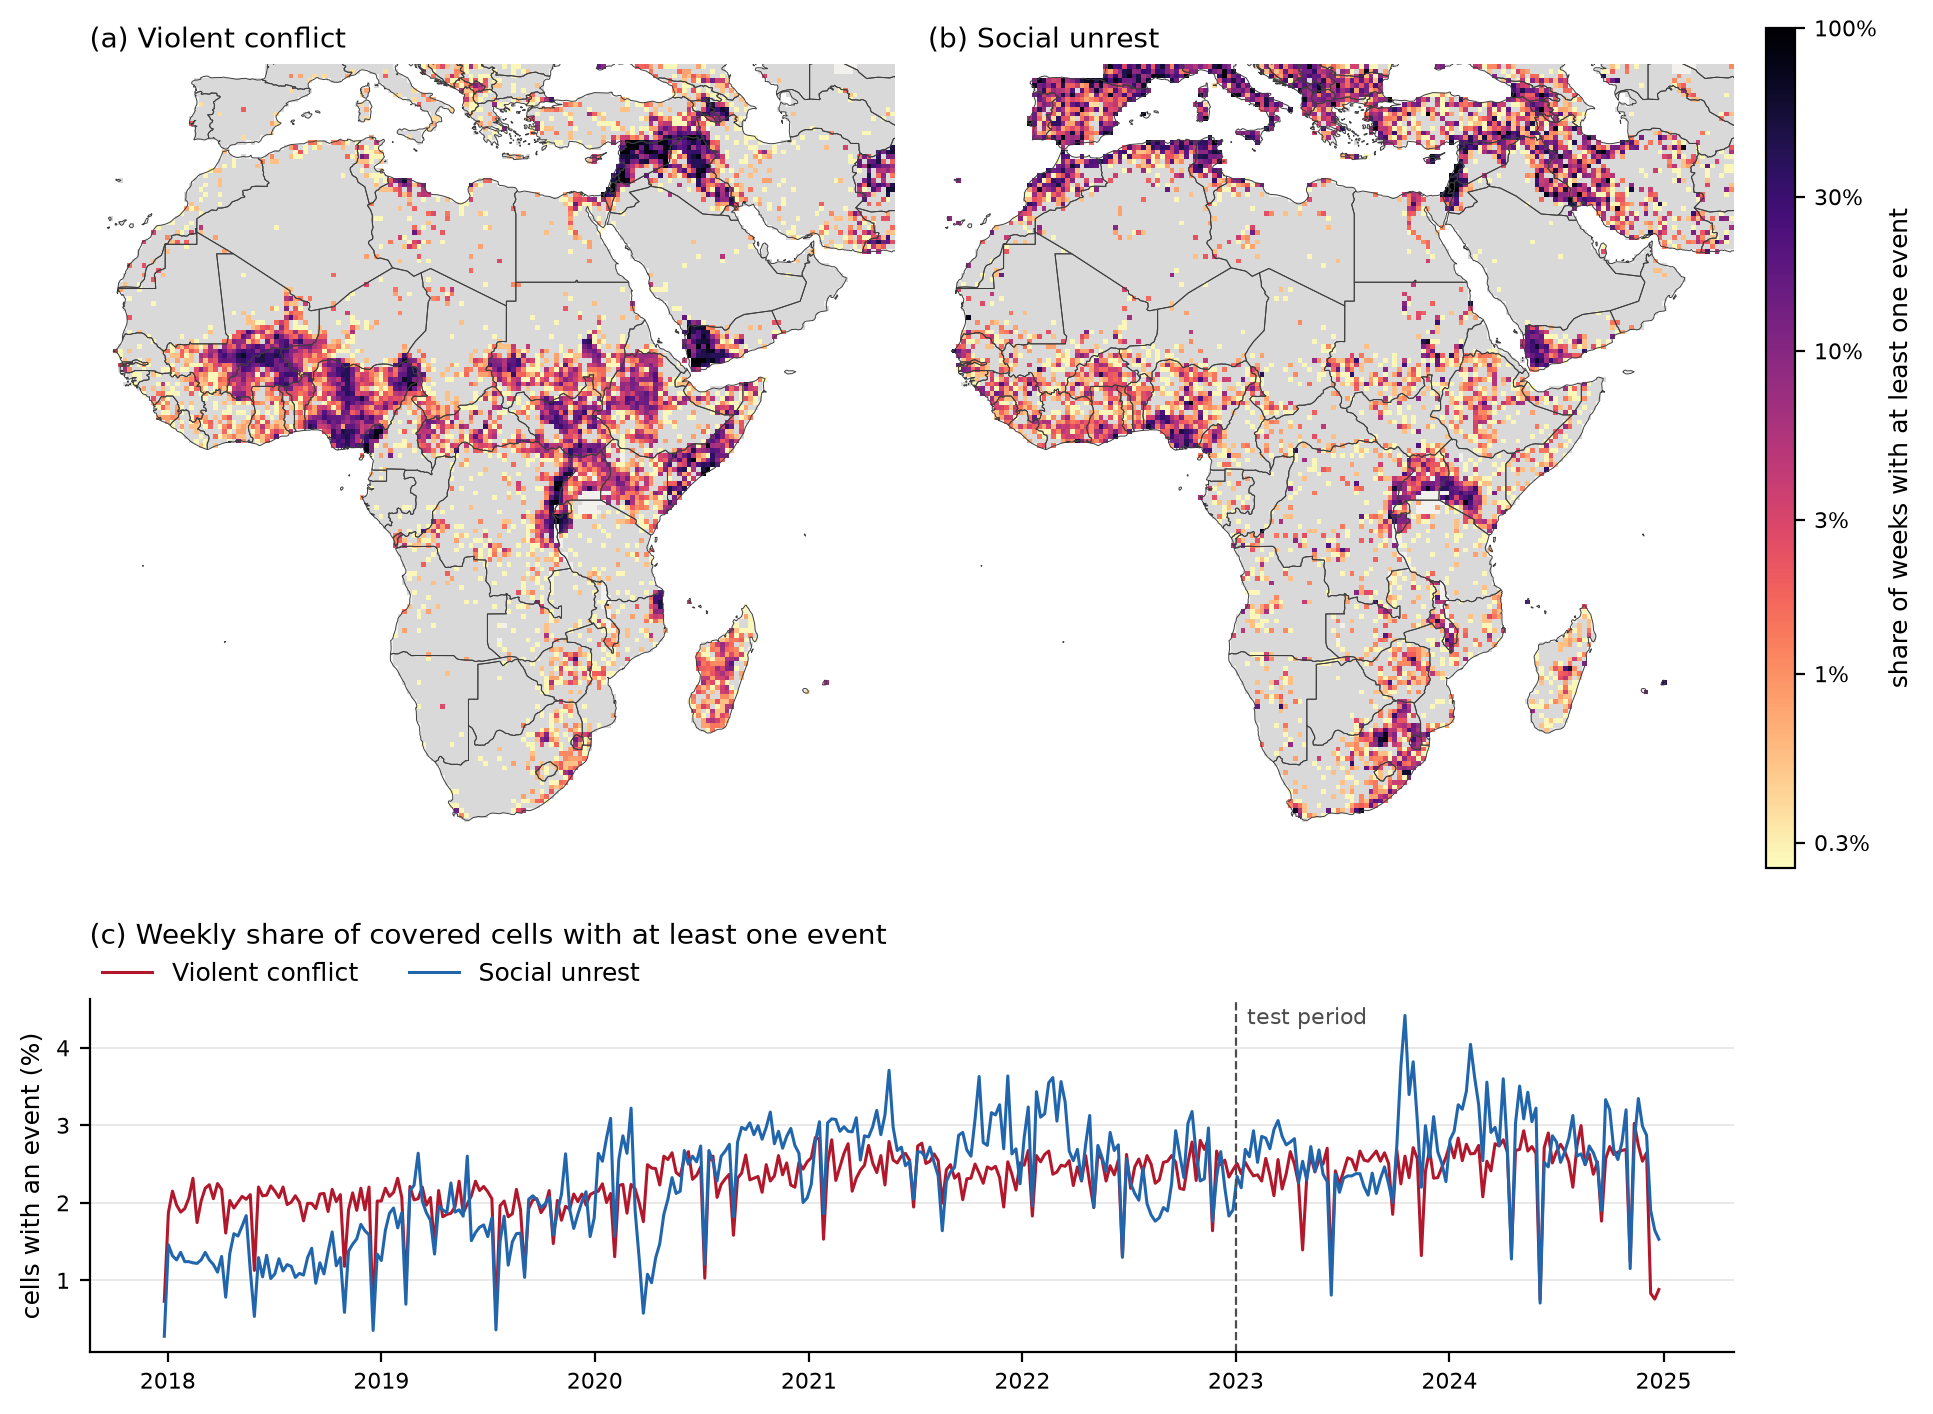
\includegraphics[width=\textwidth]{figures/data_events.png}
\caption{ACLED events on the $0.5^\circ$ grid in the AME region (Africa, the Middle
East and adjacent regions), 2018--2024, over covered cell-weeks. (a, b) Share of weeks with at least one event in
each cell, for violent conflict and social unrest (logarithmic colour scale); grey cells
have no event week. (c) Weekly share of covered cells in the region with at least one
event. The dashed line marks the start of the test period.}\label{fig:data}
\end{figure}

The grid consists of the $0.5^\circ$ cells that intersect a country, excluding cells
without a terrestrial biome. Cell-weeks in a country before its ACLED coverage start
are unobserved, not event free, and are removed. Since the probability that an event
is recorded depends on media and partner density, the outcome combines occurrence
and reporting \citep{weidmann2016closer}; the latent fields of
Section~\ref{sec:methods} absorb spatially smooth reporting differences together with
unmeasured drivers of risk, and we interpret them accordingly. The construction of the
table, including the repair of duplicated cell-weeks in the original pipeline, is
described in Section~\ref{supp:data-table} of the Supplementary Material.

\subsection{Recent event history}\label{sec:data-history}

For each cell and week we compute the number of events of each type in the four
preceding weeks, $L^{(j)}_{st} = \sum_{l=1}^{4} N^{(j)}_{s,t-l}$, using only past
weeks of the same cell. In the models of Section~\ref{sec:methods} the history enters
through $h_{st} = \log\bigl(1 + \sum_{j \in \mathcal{J}} L^{(j)}_{st}\bigr)$ for the
outcome being modelled, and through the corresponding quantity for the other outcome
as an additional covariate. Cell-weeks whose four-week history is incomplete, at the
start of the series and of each country's coverage, are dropped from the parametric
latent models. The boosting models, and the boosting offset of the hybrid models,
keep these rows and receive the incomplete history as missing.

\subsection{Environmental, socioeconomic and national covariates}\label{sec:data-cov}

Covariates are listed in Table~\ref{tab:covariates}. They vary at three
resolutions, which is central to the identification arguments of
Section~\ref{sec:methods-confounding}:
\begin{enumerate}
\item \emph{cell--week}: daily minimum and maximum temperature, heat index and
wet-bulb globe temperature (CHIRTS), precipitation (CHIRPS), PM$_{2.5}$ (CAMS) and a
drought index (Global Drought Observatory);
\item \emph{cell}: population (GHSL), river length and lake area (Natural Earth),
malaria risk (Malaria Atlas Project), terrestrial biome (RESOLVE Ecoregions) and,
in the boosting models only, an indicator of $|\mathrm{latitude}| < 30^\circ$;
\item \emph{country--year}: GDP per capita, access to electricity, the
Environmental Performance Index (EPI), the V-Dem liberal democracy index, and
per-capita greenhouse gas emissions, material footprint and ecological footprint.
\end{enumerate}
Food insecurity, the population in each IPC phase, is available for subnational
regions and periods and is apportioned to cells by population share.

Climate variables enter as their means over the four weeks before the current week,
as standardised anomalies with respect to a cell- and calendar-month-specific
climatology of the training years 2018--2022. Covariates are standardised with
training-period means; missing values are set to zero and a missingness indicator
enters for each national indicator and for IPC. Missingness is substantial (IPC phases
62.7\% of rows, PM$_{2.5}$ 55.5\%, GDP 3.6\%) and unlikely to be at random.
Section~\ref{supp:data-cov} of the Supplementary Material lists the covariates and
sources (Table~\ref{tab:covariates}) and details the anomalies and missing values.


\section{Methods}\label{sec:methods}

\subsection{A latent Gaussian model for event occurrence}\label{sec:methods-model}

Let $\mathcal{S}$ be the set of $n$ grid cells, $c(s)$ the country and $b(s)$
the biome of cell $s$, and $t = 1, \dots, T$ the weeks. Conditionally on a set
of latent effects, the outcomes are independent Bernoulli variables,
$Y_{st} \mid \pi_{st} \sim \mathrm{Bernoulli}(\pi_{st})$, with
\begin{equation}\label{eq:model}
\logit \pi_{st}
= \bx_{st}^\top \bbeta
+ \delta\, h_{st}
+ \sum_{k \in \mathcal{K}} z_{k,st}\, \beta_k(s)
+ \bz_{c(s),t}^\top \bm{\alpha}
+ u_{c(s)} + w(s) + e_s + v(s,t).
\end{equation}
Here $h_{st}$ is the recent event history of Section~\ref{sec:data-history},
so $\delta$ measures state dependence (Section~\ref{sec:methods-persistence}).
The vector $\bx_{st}$ holds the cell and cell-week covariates with fixed effects.
In the application these are the other outcome's event history, population,
malaria risk, the IPC phase 3+ population, river length and lake area, the climate
anomalies and climatologies of Section~\ref{sec:data-cov}, biome effects and year
effects. The variables $z_{k,st}$, $k \in \mathcal{K}$, are climate anomalies whose
effects $\beta_k(s)$ vary in space (Section~\ref{sec:methods-svc}); in the
application $\mathcal{K}$ contains maximum temperature only. The vector
$\bz_{ct}$ holds the national indicators with effects $\bm{\alpha}$
(Section~\ref{sec:methods-confounding}). GDP per capita is one of them: it is
national GDP divided by national population and enters as its logarithm. The
country effects $u_c \sim \Normal(0, \sigma_u^2)$ are independent, $w$ is a
Mat\'ern field on the sphere (Section~\ref{sec:methods-spde}), the cell effects
$e_s \sim \Normal(0, \sigma_e^2)$ are independent, and $v$ is a space-time field
(Section~\ref{sec:methods-st}). The four latent terms capture persistent
\emph{recorded} risk at four scales. Each mixes occurrence with reporting
(Section~\ref{sec:data-acled}): national institutions and reporting regimes ($u$),
regional hotspots that cross borders ($w$), single cells such as a town, a mine or
a border crossing ($e$), and slowly evolving episodes ($v$). The cell effect is
needed because a field with $\nu = 1$ and a range of several cells cannot represent
risk that differs between adjacent cells. Without it, such risk would be absorbed
by $w$ or by the history term $\delta h_{st}$ (Section~\ref{sec:methods-persistence}).

Missing covariate values are kept as missing through the construction of the
features. In particular, a cell-week without an IPC assessment has a missing IPC
value, not a food-insecure population of zero. After standardisation, missing values
are set to the training-period mean, and a missingness indicator is added as a
further fixed effect for each covariate group: one indicator for each national
indicator and one for IPC. Without these indicators, the imputed value would be
confounded with the fact of not being assessed, which is itself associated with
conflict. The boosting models receive the missing values as such, since XGBoost
handles them natively.

Model~\eqref{eq:model} is a latent Gaussian model \citep{rue2009inla}. Stacking all
latent quantities into
$\bm{\xi} = (\bbeta, \delta, \bgamma, \bm{\alpha}, \bu, \bw, \bm{e}, \bmeta, \bv)$, the
linear predictor is $\bm{\eta} = \bm{o} + \bA \bm{\xi}$ for a sparse design
matrix $\bA$ and an optional offset $\bm{o}$, and
$\bm{\xi} \mid \btheta \sim \Normal\{\bm{0}, \bQ(\btheta)^{-1}\}$ with a sparse,
block-diagonal precision whose blocks are listed in Table~S1 of the Supplementary Material
\citep{rue2005gmrf}. Fixed effects receive vague $\Normal(0, 10^4)$ priors and are
integrated out together with the random effects.

\subsection{Mat\'ern fields on the sphere via a finite-volume SPDE}\label{sec:methods-spde}

Following \citet{lindgren2011spde}, a Gaussian field $w$ on $\sphere$ with
Mat\'ern-like covariance is defined as the stationary solution of
\begin{equation}\label{eq:spde}
\tau\,(\kappa^2 - \Delta_{\sphere})\, w(s) = \mathcal{W}(s), \qquad s \in \sphere,
\end{equation}
where $\Delta_{\sphere}$ is the Laplace--Beltrami operator and $\mathcal{W}$ is
Gaussian white noise \citep[see also][]{lindgren2022spde}. This is the $\alpha = 2$
case, which corresponds to Mat\'ern smoothness $\nu = 1$ in the planar limit. The
field then has practical range $\rho = \sqrt{8}/\kappa$ and marginal variance
$\sigma^2 = 1/(4\pi\kappa^2\tau^2)$, provided $\rho$ is small relative to the
Earth's radius $R$. We parameterise the field by $(\rho, \sigma)$, in kilometres and
logit units.

The grid cells are natural control volumes, so instead of a triangulated mesh
we discretise \eqref{eq:spde} by finite volumes on the longitude--latitude
lattice itself \citep[for finite-volume SPDE discretisations on regular grids,
see][]{fuglstad2015exploring}. Integrating \eqref{eq:spde} over cell $A_i$ and
applying the divergence theorem with a two-point flux approximation gives
\[
\tau\Bigl\{\kappa^2 a_i w_i + \sum_{j \sim i} \frac{\ell_{ij}}{d_{ij}}(w_i - w_j)\Bigr\}
= \mathcal{W}(A_i) \sim \Normal(0, a_i),
\]
where $a_i$ is the area of cell $i$, $j \sim i$ ranges over the cells sharing an
edge with $i$, $\ell_{ij}$ is the length of the shared edge and $d_{ij}$ the
great-circle distance between the centres. For a grid with spacings
$\Delta\lambda, \Delta\varphi$ and centre latitude $\varphi_i$,
\begin{align*}
a_i &= R^2 \Delta\lambda\,\{\sin(\varphi_i + \Delta\varphi/2) - \sin(\varphi_i - \Delta\varphi/2)\},\\
\ell_{ij}/d_{ij} &= \Delta\varphi / (\cos\varphi_i\, \Delta\lambda) \quad \text{(east--west neighbours)},\\
\ell_{ij}/d_{ij} &= \cos\varphi_{ij}\,\Delta\lambda / \Delta\varphi \quad \text{(north--south neighbours)},
\end{align*}
with $\varphi_{ij}$ the latitude of the shared edge. Writing
$\bC = \mathrm{diag}(a_i)$ and $\bG$ for the weighted graph Laplacian with edge
weights $\ell_{ij}/d_{ij}$, we get $\tau \bK \bw = \bC^{1/2}\bm{\epsilon}$ with
$\bK = \kappa^2 \bC + \bG$ and $\bm{\epsilon} \sim \Normal(\bm{0}, \bm{I})$, so
\begin{equation}\label{eq:Qs}
\bw \sim \Normal\{\bm{0}, \bQ_s^{-1}\}, \qquad
\bQ_s(\rho, \sigma) = \tau^2 \bK \bC^{-1} \bK,
\qquad
\log|\bQ_s| = 2n\log\tau + 2\log|\bK| - \textstyle\sum_i \log a_i .
\end{equation}
$\bQ_s$ has at most 13 non-zeros per row. The construction is the lumped-mass
finite-volume analogue of the finite-element representation in
\citet{lindgren2011spde}. Because it uses the physical cell geometry, it accounts
for the shrinking east--west spacing towards the poles. It can also be restricted to
land cells by deleting rows and columns, and it wraps around in longitude for global
analyses. The continuum relations between $(\kappa, \tau)$ and $(\rho, \sigma)$
hold on the lattice only when $\rho$ spans several cells. A fitted range below two
or three cells (100--150\,km) indicates a field that the $0.5^\circ$ lattice does
not resolve; its $\hat\sigma$ is then not the marginal standard deviation, and we
interpret such fields as cell-level effects.

\begin{remark}\label{rem:boundary}
The discretisation imposes reflecting (Neumann) conditions on the boundary of the
lattice, which roughly doubles the marginal variance of boundary cells
\citep[Section~\ref{sec:sim-engine}; see][for the effect of boundary conditions on
SPDE fields]{khristenko2019boundary}. For a land grid the boundaries are the
coastlines. Extending the lattice into the sea removes the inflation but lets
correlation leak across narrow seas, for example between Yemen and Somalia across the
Gulf of Aden, which is substantively wrong for conflict risk. We therefore use the
barrier model of \citet{bakka2019barrier}: the SPDE is written as
\[
u(s) - \nabla\cdot\Bigl\{\tfrac{r(s)^2}{8}\nabla u(s)\Bigr\} = r(s)\sqrt{\pi/2}\,\sigma\,\mathcal{W}(s),
\]
which reduces to \eqref{eq:spde} with $\kappa = \sqrt{8}/\rho$ when
$r(s) \equiv \rho$. The lattice is extended by six rings of cells (3$^\circ$)
without data. Sea cells, identified from the Natural Earth country polygons, get
range $r(s) = f\rho$. Land cells without data, such as those outside a regional
analysis box, keep the range $\rho$, so that the field is not artificially
decorrelated at the edge of the region. The finite-volume form is
$\bK\bu = \bm{D}\bm{\epsilon}$ with $\bK = \bC + (\rho^2/8)\bG_m$, where $\bG_m$
has edge weights $2m_im_j/(m_i + m_j)\cdot\ell_{ij}/d_{ij}$, $m_i = r_i^2/\rho^2$
(the harmonic mean, the usual two-point flux choice for a discontinuous
coefficient), and $\bm{D} = \mathrm{diag}\{r_i\sigma(\pi a_i/2)^{1/2}\}$, so that
$\bQ_s = \bK\bm{D}^{-2}\bK$. Table~S2 of the Supplementary Material reports the marginal variance
at the coast and the correlation across straits of two to six cells for several
choices of $f$, at $\rho = 400$\,km. At this range, $f = 0.1$, the value of
\citet{bakka2019barrier}, gives a barrier range of 40\,km, less than one cell, and
the coastline behaves almost like a reflecting boundary. We use $f = 0.5$. At
$\rho = 400$\,km it keeps the coastal variance within about 30\% of nominal and the
correlation across straits of four cells or more (about 220\,km) below 0.04, while
a strait of two cells still has a correlation of 0.16. Straits narrower than one
cell are not resolved at this grid resolution. These figures depend on $\rho$,
because the barrier range $f\rho$ and the buffer of six rings scale differently with
it. For the fitted ranges of $w$ in the application, which are well below 400\,km,
the barrier is stronger than in Table~S2 of the Supplementary Material. For ranges of 800\,km or
more, which the SVC fields of Section~\ref{sec:methods-svc} can reach, $f\rho$
exceeds the buffer, so the coastal variance inflation returns and correlation leaks
across the wider straits. The stored real-data fits use the sea cells of the country
polygons as barriers.
\end{remark}

\paragraph{Priors.} We use penalised-complexity priors
\citep{simpson2017pc, fuglstad2019pc}: $P(\rho < \rho_0) = 0.05$ and
$P(\sigma > \sigma_0) = 0.01$, with $\rho_0 = 100$\,km (about two grid cells) and
$\sigma_0 = 1$. The PC prior of \citet{fuglstad2019pc} is derived for Mat\'ern
fields on $\mathbb{R}^2$; we use it as an approximation on the sphere, which is
adequate for ranges far below $R$. The country and cell effects have PC priors with
$P(\sigma_u > 1) = 0.01$ and $P(\sigma_e > 1) = 0.01$.

\subsection{Space-time persistence}\label{sec:methods-st}

The space-time term is a separable field that evolves as a first-order
autoregression of Mat\'ern innovations,
\[
\bv_\tau = \phi\, \bv_{\tau-1} + \sqrt{1-\phi^2}\,\bm{\epsilon}_\tau,
\qquad \bm{\epsilon}_\tau \sim \Normal\{\bm{0}, \bQ_s(\rho_v, \sigma_v)^{-1}\},
\]
\citep{cameletti2013pm10}, so that $\bv$ has precision
$\bQ_{\mathrm{AR}}(\phi) \otimes \bQ_s(\rho_v,\sigma_v)$, where
$\bQ_{\mathrm{AR}}$ is the tridiagonal precision of a unit-variance AR(1) process.
To control cost, $\tau$ indexes blocks of $\Delta$ weeks, and
$v(s,t) = v_{s,\lceil t/\Delta \rceil}$. We use $\Delta = 1$ and $\Delta = 4$ in the
simulations and $\Delta = 8$ in the application. The field $v$ is defined on the
observed land cells only, so it cannot link cells across the sea, and it has
reflecting boundaries at the edges of the observed region. In the models with $v$,
the static field $w$ uses the same lattice as elsewhere: the observed cells, a
buffer of six rings and sea barriers with $f = 0.5$ (Remark~\ref{rem:boundary}). The
prior on
$\operatorname{atanh}\phi$ is $\Normal(0, 1.5^2)$. Non-separable alternatives exist
\citep{lindgren2024diffusion} but are not needed for the questions asked here.

\subsection{State dependence versus persistent heterogeneity}\label{sec:methods-persistence}

Recent event counts dominated the importance rankings of the original boosting
analysis \citep{menicali2026conflicts}. Part of that dominance was an artefact of
duplicated rows (Section~\ref{sec:app-xgb}), but after correction recent history
remains the strongest single predictor. This has several explanations, which
model~\eqref{eq:model} separates only partially:
\begin{enumerate}
\item \emph{state dependence}: recorded events raise the probability of further
recorded events in the same place, through retaliation, mobilisation or the arrival
of armed groups;
\item \emph{persistent heterogeneity}: some places are simply riskier ($u$, $w$, $e$ or $v$
is large there), and past events are informative only as a proxy for that latent
risk \citep{heckman1981heterogeneity};
\item \emph{reporting dynamics}: media attention and reporting networks themselves
persist, so a place that has been reported on is more likely to be reported on
again, whatever happens there \citep{weidmann2016closer}.
\end{enumerate}
All three produce strong autocorrelation in $Y_{st}$ and a large predictive
contribution of $h_{st}$. In the conflict literature the distinction appears as
the question of whether apparent contagion between neighbouring places reflects
spillover or shared conditions \citep{buhaug2008contagion}. Self-exciting point
process models address it by decomposing intensity into a background and a
triggering component
\citep{mohler2011self, mohler2013multisource, porter2012hurdle, clark2018selfexciting,
reinhart2018review, jun2024hawkes}.

In model~\eqref{eq:model}, $\delta$ is the effect of recent recorded history
conditional on the latent persistence $u + w + e + v$, and it is identified only
under the assumed latent structure. It is conditional on heterogeneity at the scales
that are modelled. Persistent heterogeneity that none of the latent terms can
represent loads onto $\delta h_{st}$ and inflates $\hat\delta$. This is why the
cell effect $e$ is included: without it, time-invariant risk that varies between
adjacent cells could only be represented by $h_{st}$.
The space-time field $v$ is resolved at steps of $\Delta$ weeks, and $h_{st}$ covers the previous four weeks. When the two time scales are
similar, separating $\delta$ from $v$ relies on the AR(1) form, so we report
$\delta$ for several $\Delta$ (Section~\ref{sec:sim-persistence}). We therefore read
$\hat\delta$ as conditional dependence of recorded events, not as a causal contagion
effect. To limit the initial-conditions problem of dynamic random-effects models
\citep{wooldridge2005initial}, we drop weeks whose four-week history is incomplete
(the first weeks of each cell and of each country's ACLED coverage). We also add each
cell's history at its first usable week as a covariate, following
\citet{wooldridge2005initial}. This is a limited version of that device. A single
four-week window is a noisy proxy for a cell's initial state, and its coefficient
does not vary in time, whereas under the AR(1) form of $v$ the dependence of later
weeks on the initial state decays with time. The device therefore only partly
removes the initial-conditions bias.

\subsection{Spatially varying climate effects}\label{sec:methods-svc}

To assess whether climate effects differ across biomes and how much variation
remains within them, the effect of anomaly $k$ is decomposed as
\begin{equation}\label{eq:svc}
\beta_k(s) = \gamma_{k,b(s)} + \eta_k(s),
\qquad \bmeta_k \sim \Normal\{\bm{0}, \bQ_s(\rho_k, \sigma_k)^{-1}\},
\end{equation}
a spatially varying coefficient model \citep{gelfand2003svc,dambon2021svc} whose
mean is pooled by biome. The biome means $\gamma_{k,b}$ are fixed effects with the
vague prior of Section~\ref{sec:methods-model}. The field $\bmeta_k$ has PC priors
with $P(\rho_k < 100\,\mathrm{km}) = 0.05$ and $P(\sigma_k > 0.5) = 0.01$, and
$\sigma_k$ measures heterogeneity within biomes. The design of $\bmeta_k$ is the
sparse matrix with entry $z_{k,st}$ in row $(s,t)$ and column $s$.

Three summaries of a biome-specific effect should be distinguished:
\begin{itemize}
\item \emph{Fixed biome slopes.} A model with fixed biome-specific slopes and no
$\bmeta_k$ estimates an information-weighted average,
$\sum_{s \in \mathcal{S}_b}\omega_s\beta_k(s) / \sum_{s \in \mathcal{S}_b}\omega_s$,
with $\omega_s \approx \sum_t z_{k,st}^2\pi_{st}(1-\pi_{st})$. This average puts
most weight on the high-risk cells of the biome.
\item \emph{Biome means.} Model~\eqref{eq:svc} targets the biome mean $\gamma_{k,b}$,
the mean of the process that generated the biome's coefficients. This is a
superpopulation quantity. Because $\bmeta_k$ is not constrained to average zero
within biomes and biomes are large contiguous regions, $\gamma_{k,b}$ is separated
from the biome average of $\bmeta_k$ mainly when $\rho_k$ is small relative to the
size of the biome. When $\rho_k$ is comparable to biome size, the separation rests
partly on the prior. A nearly constant component of $\bmeta_k$ is then confounded
with a common shift of all $\gamma_{k,b}$. The intervals for $\gamma_{k,b}$ are
conditional on $(\hat\rho_k, \hat\sigma_k)$ (Section~\ref{sec:methods-inference}),
and in this situation the uncertainty in these hyperparameters may be the largest
source of error. They should be read with this in mind.
\item \emph{Median SHAP value.} The summary used in the SHAP-based analysis of
\citet{menicali2026conflicts}, the median SHAP value within a biome, differs from
both. The following identities are on the logit scale of the model. They hold for
interventional SHAP values when the features are independent. The path-dependent
TreeSHAP of XGBoost \citep{lundberg2020trees}, which we use, satisfies them only
approximately, and features correlated with biome, such as distance from the
equator, can absorb part of an interaction. For a feature with
an additive effect $f_k(z)$, the SHAP value is $f_k(z) - \E f_k(Z_k)$, so the median
within a biome is $\operatorname{median}_{(s,t):\, b(s) = b}\{f_k(z_{k,st}) - \E
f_k(Z_k)\}$. For a linear effect $\beta_k z$ this is $\beta_k$ times the median of
$z_{k,st} - \E z_k$ in the biome. It reflects where the biome's covariate values lie
relative to the global mean as much as the strength of the effect. When the effect
is a biome-by-feature interaction, SHAP also splits the interaction between the
feature and biome \citep{kumar2020problems,aas2021explaining}. A pure interaction
$g(b)z$, with $B$ independent of $Z$, contributes
$\{g(b) + \E g(B)\}(z - \E z)/2$ to the SHAP value of $z$. Within biome $b$, the
least-squares slope of the SHAP value of $z$ on $z$ therefore targets
$\{g(b) + \E g(B)\}/2$, which is pulled towards the average effect across biomes. It
equals $g(b)/2$ only when $\E g(B) = 0$. The SHAP value with the interaction credited
fully to $z$, $\Phi_{zz} + 2\sum_{j \neq z}\Phi_{zj}$ with $\Phi$ the SHAP
interaction values \citep{lundberg2020trees}, equals $g(b)(z - \E z)$ in this case,
so its slope within biome $b$ targets $g(b)$ whatever the mean of $g$.
\end{itemize}

\subsection{National indicators and spatial confounding}\label{sec:methods-confounding}

National indicators $\bz_{ct}$, such as GDP per capita, the EPI or the ecological
footprint, take one value per country and year. GDP per capita is computed at the
national level (Section~\ref{sec:methods-model}), so that it is constant within each
country and year like the other indicators. We decompose each into a
between-country component, its country mean over the training years
$\bar z_c$, and a within-country component $z_{ct} - \bar z_c$, with separate
coefficients (a Mundlak decomposition). Year effects absorb trends common to all
countries. The between coefficients are identified from contrasts between the
$n_c$ countries only, so their effective sample size is of order $n_c$, not the
number of cell-weeks. Modelling cell-weeks as conditionally independent, or
bootstrapping spatial blocks that cut across countries, therefore produces intervals
that are far too narrow. The within coefficients rest on the few years of change
within each country. A country with no training-period value of an indicator gets
the mean between component and a value of one for that indicator's missingness
indicator (Section~\ref{sec:methods-model}). The missingness indicator is itself
country-level, so its coefficient also rests on few contrasts.

If the indicators are associated with unobserved country-level risk, so that
$\E\{u_c + \bar w_c \mid \bar z_c\} \neq 0$ with $\bar w_c$ the country average of
$w$, then the between coefficients are confounded. An indicator of environmental
performance that tracks state capacity, or reporting capacity, is the leading
example. This is the spatial confounding problem
\citep{reich2006effects, hodges2010adding, paciorek2010importance}. Adding a spatial
random effect changes the estimate of a spatially smooth covariate's coefficient,
and in general neither the estimate with the random effect nor the one without it is
unbiased for a causal effect \citep{khan2022restricted, zimmerman2022deconfounding}.
Recent work has made this more precise. Generalised least squares with a spatial
random effect can be consistent when the covariate has non-spatial variation
\citep{gilbert2025consistency}. Confounding in the data-generating process should be
distinguished from the behaviour of the analysis model \citep{khan2026rethinking}.
The bias depends on how the covariate and the confounder are spread across spatial
scales \citep{guan2023spectral, dupont2026demystifying}. A country-constant indicator
has no within-country spatial variation, so these results give little reassurance
here.

We report the following estimators and treat their disagreement as a measure of how
fragile the national-level conclusions are:
\begin{enumerate}
\item model~\eqref{eq:model} without latent effects;
\item model~\eqref{eq:model} with $\bu$ and $\bm{e}$;
\item model~\eqref{eq:model} with $\bu$, $\bw$ and $\bm{e}$;
\item a \emph{spatial+} estimator \citep{dupont2022spatial}: model~\eqref{eq:model}
with $\bw$ and $\bm{e}$ but \emph{without} $\bu$, in which each between component is
replaced by its residual after an area-weighted projection, over the observed land
cells, on the $m$ smoothest eigenvectors $\bm{\psi}$ of
$\bG\bm{\psi} = \lambda\bC\bm{\psi}$.
\end{enumerate}
These eigenvectors are the lattice analogue of the thin-plate eigenvectors of
\citet{dupont2022spatial}. A country-constant indicator varies only by steps at
borders. After the projection, the residual keeps these steps, minus a smooth
function of the eigenvectors. In a model without $\bu$, the smooth variation is left
to $\bw$ and the border steps identify the coefficient. In a model with $\bu$, the
border steps are country-level jumps, which $\bu$ can absorb. The coefficient would
then be identified only through the shrinkage of $\bu$ under its exchangeable prior,
which is independent of the indicator. That is the random-effects exogeneity
assumption we have just called implausible. This is why (iv) omits $\bu$. Without
$\bu$, however, country-level risk that is not spatially smooth remains a possible
confounder, and the projection also gives the residual some within-country variation
that is a function of the smooth eigenvectors. We therefore treat (iv) as a
sensitivity analysis and not as a preferred estimate.

The default $m^*$ is the number of eigenvalues below
$\kappa_w^2 = 8/\hat\rho_w^2$, the eigenvectors that vary on scales longer than the
fitted range of $w$. This number can be large. By Weyl's law, for a region of area
$|D|$ it is approximately $|D|\kappa_w^2/(4\pi) = 2|D|/(\pi\hat\rho_w^2)$. If
$\hat\rho_w$ is close to the ranges of the hybrid fields of
Section~\ref{sec:app-hybrid} (264\,km for conflict and 68\,km for unrest, on 13{,}719
cells), $m^*$ is of the order of a few hundred for conflict and several thousand for
unrest. The eigenvectors near the cut-off then vary on scales comparable to the size
of many countries, and most of the between-country variation of a country-constant
indicator is projected out. We therefore report $m = 10$, $m = 20$ and $m^*$, and
state $m^*$ for each fit \todo{values of $m^*$ from the rerun of fit\_glmm.py, and
whether the eigenvalue computation reached $m^*$}. The restricted spatial regression
of \citet{reich2006effects} is not used, because its intervals are known to be
anticonservative \citep{hanks2015restricted, khan2022restricted}.

\subsection{Hybrid models: boosting offsets with latent effects}\label{sec:methods-hybrid}

To retain the flexibility of gradient boosting for the many weakly informative
covariates, we also fit a semiparametric version of~\eqref{eq:model}. Its fixed part
is replaced by the logit $\hat f(\bx_{st})$ of an XGBoost classifier
\citep{chen2016xgboost}, which enters as an offset:
\begin{equation}\label{eq:hybrid}
\logit \pi_{st} = \hat f^{(-k(s))}(\bx_{st}) + \beta_0 + u_{c(s)} + \omega(s),
\end{equation}
where $\omega$ is either the Mat\'ern field $w$ or independent cell effects. The
offset is \emph{cross-fitted by country}. Countries are assigned at random to $K = 5$
folds. For each fold $k$, $\hat f^{(-k)}$ is trained on the 2018--2022 rows of the
other folds, with its number of trees chosen by early stopping on 2022 after training
on 2018--2021. It then provides the offset for every row of fold $k$, in both the
training and test periods. The offset and the latent effects are fitted on the
Africa and Middle East box only. Trees that receive national indicators can identify
countries, and through population, biome and distance from the equator, approximate
locations. Cross-fitting by country ensures that the offset of a cell was learned
without any data from its own country, so that $u$ does not count that country's
data twice. It does not exclude data from neighbouring countries. The offset of a
cell near a border can be learned from the outcomes of cells across the border, and
$\omega$ is estimated from the residuals of those same cells. Regional hotspots that
cross borders can therefore enter both the offset and $\omega$. The fitted $\omega$
is a residual field. Its range and standard deviation are not comparable with those
of $w$ in model~\eqref{eq:model}. The offset enters with its coefficient fixed at
one, so fold models whose logits are over- or under-dispersed are not rescaled; $u$
absorbs shifts between folds but not differences in scale. Inference for $u$ and
$\omega$ is conditional on the offset, whose estimation uncertainty is not
propagated, so their posterior uncertainty is understated. Cross-fitting is used here
in the loose sense of sample splitting, not with an orthogonal score as in
\citet{chernozhukov2018dml}.

The price of cross-fitting is that the offset is weaker than a boosting model trained
on all locations. The cross-fitted XGBoost model never sees the country it predicts,
while $u$ and $\omega$ are estimated from that country's training data. A gain of the
hybrid model over the cross-fitted offset alone is therefore not evidence that the
latent effects add anything. The hybrid models are compared, on identical test rows,
with the corrected boosting model trained on all locations, with the location-aware
boosting baseline, with each other ($\omega$ as a field or as independent cell
effects) and with the persistence baseline (Section~\ref{sec:methods-diagnostics}).
The offset uses the same rows, features and hyperparameters as the corrected
boosting model (Section~\ref{sec:app-xgb}). It is trained without class weights, so
it is on the log-odds scale.

Model~\eqref{eq:hybrid} differs from GPBoost \citep{sigrist2022gpboost,
sigrist2023lagaboost}, which alternates boosting steps with latent Gaussian model
updates: here the boosting fit is fixed before the latent model is fitted. This
makes the model cheap enough for the global data and allows the same Laplace
machinery to be used. Random forests with spatially correlated errors
\citep{saha2023rfgls} are a further alternative.

The boosting analysis of \citet{menicali2026conflicts} trained XGBoost with positives
weighted by $\omega_+ = (n_0/n_1)^{1/2}$. For the unrestricted minimiser of the
logistic loss, this shifts the fitted log-odds by $\log\omega_+$
\citep{king2001rare}. We therefore prior-correct the predictions of the weighted
models, $\hat f \leftarrow \hat f - \log\omega_+$, before probabilistic scoring. For
boosted trees the correction is only approximate, because the weights also act on
the leaf penalty, on the minimum leaf weight, which is defined on weighted Hessians,
and on early stopping. The scores of the weighted models therefore include any
remaining miscalibration. Class reweighting does not improve discrimination and
miscalibrates probabilities \citep{vandengoorbergh2022harm}, and the corrected
boosting model is trained without it (Section~\ref{sec:app-xgb}).

\subsection{Inference}\label{sec:methods-inference}

For fixed hyperparameters $\btheta$, the posterior mode
$\bm{\xi}^* = \arg\max_{\bm{\xi}}\{\log p(\bm{y}\mid\bm{\xi}) - \tfrac12 \bm{\xi}^\top \bQ \bm{\xi}\}$
is found by damped Newton iterations,
\[
\bm{\xi} \leftarrow \bm{\xi} + \lambda\,(\bQ + \bA^\top \bm{W} \bA)^{-1}
\{\bA^\top(\bm{y} - \bm{\pi}) - \bQ\bm{\xi}\},
\qquad \bm{W} = \mathrm{diag}\{\pi_{st}(1-\pi_{st})\},
\]
with step halving. The Laplace approximation to the marginal likelihood is
\begin{equation}\label{eq:laplace}
\log \tilde p(\bm{y}\mid\btheta) = \log p(\bm{y}\mid\bm{\xi}^*)
- \tfrac12 \bm{\xi}^{*\top}\bQ\bm{\xi}^* + \tfrac12\log|\bQ| - \tfrac12\log|\bQ + \bH|,
\qquad \bH = \bA^\top\bm{W}^*\bA .
\end{equation}
The hyperparameters are set to
$\hat\btheta = \arg\max\{\log\tilde p(\bm{y}\mid\btheta) + \log p(\btheta)\}$ by
L-BFGS-B with finite-difference gradients on the internal scale (logarithms of ranges
and standard deviations, $\operatorname{atanh}\phi$). Each evaluation warm-starts
Newton at the previous mode. Given $\hat\btheta$, the latent posterior is approximated
by $\Normal\{\bm{\xi}^*, (\bQ + \bH)^{-1}\}$. Samples reuse the factorisation of
$\bQ + \bH$ already computed at the mode, through the perturbation identity
\[
\bm{\xi} = \bm{\xi}^* + (\bQ + \bH)^{-1}\bigl(\bm{R}^\top\bm{\epsilon}_1 + \bA^\top\bm{W}^{*1/2}\bm{\epsilon}_2\bigr),
\]
where $\bm{R}^\top\bm{R} = \bQ$ is block-wise explicit, for instance
$\bm{R} = \bm{D}^{-1}\bK$ for a Mat\'ern block and a Kronecker product of a
bidiagonal AR(1) factor with that matrix for $\bv$. This is an empirical Bayes
version of INLA \citep{rue2009inla} and is similar in spirit to TMB
\citep{kristensen2016tmb}. Laplace approximations are generally accurate for
binary GLMMs but can understate uncertainty when there are few observations per
latent variable and events are rare \citep{fong2010glmm, ferkingstad2015improving}.
The intervals also ignore the uncertainty in $\hat\btheta$.
Section~\ref{sec:sim-engine} therefore checks coverage at the event prevalence of
the data, and Section~\ref{sec:sim-persistence} checks it for the space-time model,
where each latent value is informed by only $\Delta$ Bernoulli observations.

\paragraph{Computation.} All matrices are sparse. Every Newton step and every
log-determinant requires a sparse factorisation of $\bQ + \bH$, whose sparsity
pattern does not depend on $\btheta$. We use a sparse LU factorisation in symmetric
mode (SuperLU). For matrices of dimension above 2{,}000, the fill-reducing ordering
is a nested dissection computed by METIS \citep{karypis1998metis}; it is computed
once and reused, but the factorisation itself is recomputed at every Newton step and
every evaluation of~\eqref{eq:laplace}. If METIS is not available, the code falls
back to multiple minimum degree on $\bm{A}^\top + \bm{A}$. For the space-time model
the nested-dissection ordering reduced factorisation time by a factor of 7 to 14
compared with that fallback. An LU factorisation stores both triangular factors, so
it needs about twice the memory of a Cholesky factor of the same matrix. Newton
iterations stop after at most 50 steps, and a value of $\btheta$ at which the
factorisation fails is given a very low objective value. Both events can make the
optimiser stop at a poor point, so they should be recorded for each fit
\todo{report Newton non-convergence and failed evaluations for the real-data
fits}. Since $\bH = \bA^\top\bm{W}\bA$ aggregates over weeks, the
cost of the spatial and SVC blocks is driven by the number of cells, not by the
number of cell-weeks. A global $0.5^\circ$ land grid gives about $6\times10^4$
latent values per spatial field. The space-time block has $nT_v$ latent values,
which is why it is fitted on a regional subset. The fixed-effect and country columns
add dense rows to $\bQ + \bH$; with tens of fixed effects their cost is small.

\paragraph{Prediction.} For a new cell-week with design row $\bm{a}$ and
offset $o$, the posterior predictive probability is
$\E\{\expit(o + \bm{a}^\top\bm{\xi})\} \approx \expit\{m/\sqrt{1 + \pi s^2/8}\}$, where
$m$ and $s^2$ are the posterior mean and variance of $o + \bm{a}^\top\bm{\xi}$; $s^2$
is estimated from posterior samples. Test years beyond the training period take the
year effect of the last training year.

\subsection{Diagnostics and evaluation}\label{sec:methods-diagnostics}

\paragraph{Residual diagnostics.} Binary residuals are uninformative one at a
time, so we aggregate over the test weeks within cells. The standardised cell
residual is
\[
r_s = \sum_{t} (y_{st} - \hat\pi_{st}) \Big/ \Bigl\{\sum_t \hat\pi_{st}(1-\hat\pi_{st})\Bigr\}^{1/2},
\]
with the sums over the test period 2023--2024. All residual diagnostics reported in
the paper are computed in this way for every model, including the cross-fitted
offset, on the same test rows. Residuals of in-sample latent-model fits are shrunk
and spatially dependent through the smoother, and we do not use training-period
residuals as evidence.

Even for a correct model, the test residuals are neither standard normal nor
independent across cells. The predictions $\hat\pi_{st}$ carry the estimation error
of the training period, for example in $\hat w(s)$. A logit error $\epsilon_s$
contributes about $\epsilon_s\{\sum_t \pi_{st}(1-\pi_{st})\}^{1/2}$ to $r_s$, which
grows with the number of test weeks, and the errors of a smoothed field are
positively correlated between neighbours. The diagnostics below are therefore used
to compare models on the same rows, not as tests against a null of independence. We
report:
\begin{itemize}
\item Moran's $I$ \citep{moran1950notes} of $\{r_s\}$ for rook adjacency. We also give
a permutation $p$-value from $B = 999$ permutations, which is bounded below by
$1/(B + 1)$. Its null hypothesis of exchangeable residuals does not hold even for a
correct model, so it is descriptive only;
\item the empirical semivariogram of $\{r_s\}$ against great-circle distance;
\item the correlation of $r_s$ between neighbouring cells in the same country and
across a border.
\end{itemize}
A larger within-country correlation can point to effects at the country level, of
occurrence or of reporting. For the cross-fitted offset it also has a mechanical
source. Neighbours in the same country are always predicted by the same fold model,
while neighbours across a border are usually predicted by different fold models,
whose differences create a country-level residual component. For this model we
therefore also split the across-border pairs into pairs whose two countries are in
the same fold and pairs in different folds.

\paragraph{Out-of-sample evaluation.} Models are trained on 2018--2022 and
evaluated on 2023--2024, matching the original analysis. All models are compared on
identical test rows. We report the logarithmic score and the Brier score, both
strictly proper \citep{gneiting2007strictly}, and the area under the
precision--recall curve, computed as average precision \citep{boyd2013area}. The
latter is more informative than the ROC curve at the low prevalence of the data
\citep{saito2015precision}. Paired differences in log score and Brier score are
reported with two standard errors: one clustered by cell and one clustered by
country, with the number of clusters. The cell-clustered errors allow for dependence
over time within a cell but not between cells. The latent fields and the national
indicators induce dependence at regional and national scales
(Section~\ref{sec:methods-confounding}), so the country-clustered errors are the
more reliable of the two, although they rest on few clusters. Since prediction in
the same places is dominated by persistence \citep{mueller2022hard}, every model is
compared with a persistence baseline that ranks cell-weeks by the number of events in
the previous four weeks. We also report all scores on \emph{onset} rows: test
cell-weeks in cells that had no event of that outcome in the previous 52 weeks. On
these rows recent history carries no information, so they show how well a model
anticipates events in places that have been quiet.

We also compare every model with a \emph{location-aware} boosting baseline that adds
each cell's training-period event rate as a feature. For the fit used to choose the
number of trees by early stopping on 2022, this rate is computed from 2018--2021
only, so it uses no 2022 outcomes. For the final fit on 2018--2022 it is computed
leaving out the row's own year, and for the test rows it is the rate over
2018--2022. This baseline is the boosting counterpart of a cell intercept, and the
latent fields have to improve on it to be worth their cost.

\section{Simulation studies}\label{sec:simulation}

We use simulation to answer five questions that the application raises but
cannot settle on its own:
(S0) whether the finite-volume SPDE and the empirical Bayes Laplace
approximation recover the field and give calibrated intervals;
(S1) whether residual spatial structure left by a boosting model can be
detected and modelled, and whether modelling it improves forecasts;
(S2) how national indicators behave under spatial confounding;
(S3) whether state dependence can be separated from persistent heterogeneity;
(S4) whether biome-specific climate effects are recovered better by spatially
varying coefficients than by SHAP summaries.
All code is in the supplementary material.

\subsection{Data-generating process}\label{sec:sim-dgp}

The simulator mimics the structure of the ACLED grid. The domain is a
$40 \times 30$ block of $0.5^\circ$ cells between $10^\circ$E and $30^\circ$E and
between $5^\circ$S and $10^\circ$N (1{,}200 cells of about 55\,km), with 104
training weeks, 52 test weeks and 12 burn-in weeks. Countries are the Voronoi
cells of randomly placed seeds (14 countries; 25 in S2). Four biomes are
latitude bands with boundaries perturbed by a smooth random field, ordered from
``cold'' (biome 1) to ``tropical'' (biome 4). Population is a standardised
Mat\'ern field (range 250\,km) plus white noise. Temperature and precipitation
anomalies are standardised AR(1) processes in time (coefficients 0.6 and 0.3) of
Mat\'ern fields with ranges of 800 and 500\,km. Three national covariates
$Z_0, Z_1, Z_2$ are standard normal across countries; $Z_1$ and $Z_2$ have no
effect but, like the national indicators in the data, allow trees to identify
countries. Outcomes are generated sequentially from
\begin{equation}\label{eq:sim}
\logit\pi_{st} = \beta_0 + \beta_{\mathrm{pop}}\mathrm{pop}_s
+ \delta\log\Bigl(1 + \textstyle\sum_{l=1}^{4} y_{s,t-l}\Bigr)
+ \beta(s)\,\mathrm{temp}_{st} + \beta_{\mathrm{prec}}\mathrm{prec}_{st}
+ \alpha Z_{0,c(s)} + u_{c(s)} + w(s) + v(s,t),
\end{equation}
with $\beta(s) = \gamma_{b(s)} + \eta(s)$, $u_c \sim \Normal(0, 0.3^2)$, and
$w$, $\eta$ and $v$ drawn from the GMRFs of Section~\ref{sec:methods}. Unless
stated otherwise, $\beta_0 = -4$, $\beta_{\mathrm{pop}} = 0.5$, $\delta = 0.6$,
$\bgamma = (-0.3, -0.1, 0.1, 0.3)$, $\eta \equiv 0$, $\beta_{\mathrm{prec}} = -0.15$,
$\alpha = 0$, $\sigma_w = 1$, $\rho_w = 400$\,km and $v \equiv 0$. The resulting
prevalence of event weeks is 3--4\%, close to that of the data. Spatial
confounding (S2) is induced by setting
$Z_{0,c} = \varrho\,\tilde\ell_c + (1-\varrho^2)^{1/2}\epsilon_c$, where
$\tilde\ell_c$ is the standardised country average of $u_c + w(s)$ and
$\epsilon_c \sim \Normal(0,1)$.

The boosting model is XGBoost with the hyperparameters of the original analysis \citep{menicali2026conflicts}
(depth 5, learning rate 0.05, row and column subsampling 0.8, minimum child
weight 30, $L_2$ penalty 5; 300 rounds), without class weights. Its features
are population, distance from the equator, biome, the two anomalies, $Z_0$--$Z_2$
and the four-week event count. As in the original analysis, the features
include no coordinates.

\subsection{S0: accuracy of the field representation and of the Laplace engine}\label{sec:sim-engine}

We simulate $w$ from the lattice SPDE~\eqref{eq:Qs} on the $40 \times 30$ domain
with $\rho_w = 400$\,km and $\sigma_w = 1$, and Bernoulli outcomes for 40 weeks
from $\logit\pi_{st} = -2 + 0.5\,x_{st} + w(s)$ with $x_{st} \sim \Normal(0,1)$,
50 replicates. Table~\ref{tab:s0} summarises the results. Across 2{,}000
draws, the empirical marginal variance of the field is 1.07 in cells at least
eight cells (about 440\,km) from the edge of the domain, against a nominal 1.
At the edge it is 2.02, the doubling induced by the Neumann boundary that
motivates the buffer of Remark~\ref{rem:boundary}. The hyperparameters are
recovered with little bias ($\hat\rho_w = 399$\,km, $\hat\sigma_w = 0.99$),
and the posterior mean of $w$ has correlation 0.96 with the truth. Plug-in 95\%
intervals cover $0.5$ in 92\% of replicates (Monte Carlo SE 3.8\%) and cover
$-2 + w(s)$ for 94.4\% of cells, so ignoring the uncertainty in $\btheta$ costs
little here. A fit takes about 5 seconds on one core.

\begin{table}
\caption{S0: accuracy of the finite-volume SPDE field and of the empirical
Bayes Laplace approximation (50 replicates).}\label{tab:s0}
\centering\small
\begin{tabular}{@{}lcc@{}}
\toprule
Quantity & common ($b_0=-2$, 50 reps) & rare ($b_0=-4.5$, 50 reps) \\
\midrule
Prevalence of event weeks & 0.161 (0.030) & 0.019 (0.005) \\
$\hat\rho_w$ (km) [truth 400] & 420 (40) & 409 (51) \\
$\hat\sigma_w$ [truth 1] & 0.884 (0.064) & 0.875 (0.075) \\
$\hat b_1$ [truth 0.5] & 0.494 (0.016) & 0.502 (0.021) \\
Coverage of 95\% interval for $b_1$ & 0.88 (0.05) & 0.96 (0.03) \\
Coverage of 95\% intervals for $b_0 + w(s)$ (share of cells) & 0.948 (0.009) & 0.943 (0.017) \\
$\mathrm{cor}(\hat w, w)$ & 0.954 (0.008) & 0.914 (0.018) \\
Fit time (s) & 2.4 (0.7) & 3.4 (0.8) \\
Marginal variance of $w$, interior cells [nominal 1] & 1.07 & -- \\
Marginal variance of $w$, edge cells & 2.02 & -- \\
\bottomrule
\end{tabular}

\end{table}

\subsection{S1: residual structure after boosting}\label{sec:sim-residual}

Data are generated from \eqref{eq:sim} with the default parameters, and the
models are trained on the first 104 weeks and evaluated on the following 52,
as in the original analysis. Table~\ref{tab:s1} reports
out-of-sample scores over 20 replicates and Table~\ref{tab:s1-field} the
residual diagnostics and the recovery of the field. Figure~\ref{fig:s1} shows
one replicate.

Three findings stand out. First, boosting does not absorb the residual field
even with in-sample training on the same locations. Moran's $I$ of the cell
residuals of the XGBoost model as used in the original analysis is 0.33
(SD 0.07 across replicates), against an expected value of about $-0.001$ under
independence. For spatially cross-fitted XGBoost it is 0.59. The trees recover
part of the field through country-identifying national covariates, which is
exactly the leakage that makes in-sample residuals understate the
spatial structure (Section~\ref{sec:methods-hybrid}). Second, the field
estimated on top of the cross-fitted offset recovers the truth well
(correlation between $\hat w$ and $w$ of 0.81 when $u$ is included), and its hyperparameters are close to
the truth: $\hat\rho_w = 373$\,km against 400 and $\hat\sigma_w = 0.94$
against 1. Third, modelling the residual field improves forecasts for the
same places. The hybrid model improves on the original XGBoost in log score
in all 20 replicates (mean difference $-0.0031$, SE $0.0003$) and in AUC-PR in 19
of 20 (mean difference $+0.011$, SE $0.001$). The correctly specified parametric
model is better still, in every replicate. The persistence baseline reaches an
AUC-PR of 0.10, against 0.27 for the true probabilities; in these simulations
persistence is a much weaker benchmark than it is likely to be in the data,
where some cells record events almost every week.

\begin{table}
\caption{S1: out-of-sample scores on the 52 test weeks (mean over 20
replicates, Monte Carlo standard error in parentheses). Lower is better for
the log and Brier scores.}\label{tab:s1}
\centering\small
\begin{tabular}{@{}lcccc@{}}
\toprule
Model & Log score & Brier & AUC-PR & AUC-ROC \\
\midrule
True probabilities & 0.1429 (0.0080) & 0.0367 (0.0026) & 0.267 (0.018) & 0.826 (0.005) \\
XGBoost (as in original analysis) & 0.1501 (0.0084) & 0.0377 (0.0027) & 0.235 (0.017) & 0.790 (0.006) \\
XGBoost, spatially cross-fitted & 0.1649 (0.0098) & 0.0402 (0.0031) & 0.152 (0.015) & 0.715 (0.008) \\
Cross-fitted XGBoost + $w$ & 0.1470 (0.0082) & 0.0374 (0.0027) & 0.245 (0.017) & 0.809 (0.005) \\
Cross-fitted XGBoost + $u + w$ & 0.1469 (0.0082) & 0.0374 (0.0027) & 0.245 (0.017) & 0.810 (0.005) \\
Parametric model with $u + w$ & 0.1457 (0.0081) & 0.0371 (0.0026) & 0.253 (0.018) & 0.814 (0.005) \\
Persistence baseline & -- & -- & 0.103 (0.009) & -- \\
\bottomrule
\end{tabular}

\end{table}

\begin{table}
\caption{S1: residual diagnostics and recovery of the field (mean and SD over
20 replicates).}\label{tab:s1-field}
\centering\small
\begin{tabular}{@{}lcc@{}}
\toprule
Quantity & Mean & SD \\
\midrule
Moran's $I$ of cell residuals, XGBoost (original) & 0.330 & 0.069 \\
Moran's $I$ of cell residuals, XGBoost cross-fitted & 0.591 & 0.064 \\
$\mathrm{cor}(\hat w, w)$, XGBoost + $w$ & 0.768 & 0.049 \\
$\mathrm{cor}(\hat w, w)$, XGBoost + $u + w$ & 0.814 & 0.036 \\
$\hat\rho_w$ (km), XGBoost + $u + w$ [truth 400] & 373.374 & 48.288 \\
$\hat\sigma_w$, XGBoost + $u + w$ [truth 1] & 0.943 & 0.095 \\
\bottomrule
\end{tabular}

\end{table}

\begin{figure}
\centering
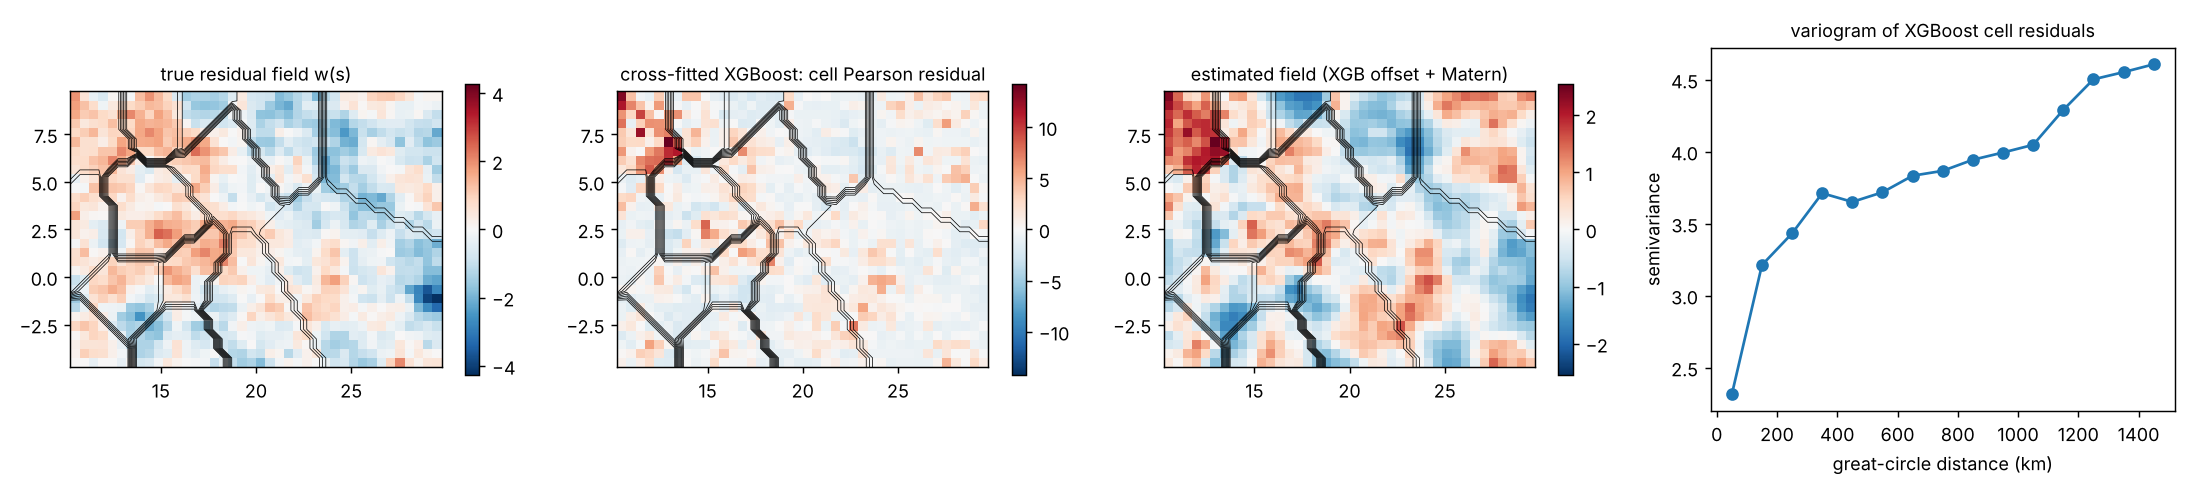
\includegraphics[width=\textwidth]{figures/s1_maps.png}
\caption{S1, one replicate. From left: the true field $w$; standardised cell
residuals of the cross-fitted XGBoost model; posterior mean of $w$ in the
hybrid model~\eqref{eq:hybrid}; semivariogram of the XGBoost cell residuals.
Lines are country borders.}\label{fig:s1}
\end{figure}

\subsection{S2: national indicators under spatial confounding}\label{sec:sim-confounding}

Three scenarios with 25 countries and 30 replicates each are considered:
no confounding with $\alpha = 0$ ($\varrho = 0$); confounding with $\alpha = 0$
($\varrho = 0.8$); and confounding with a true effect $\alpha = -0.3$. We
compare the estimators of Section~\ref{sec:methods-confounding} with the
XGBoost summary of the original analysis. For the latter, the effect of $Z_0$
is summarised by the least-squares slope of its SHAP values on $Z_0$, with
intervals from 20 replicates of the $5^\circ$ block bootstrap on a fixed 30\%
subsample of the training data, as in the original analysis.

\begin{table}
\caption{S2: estimation of the effect $\alpha$ of a national indicator (30
replicates per scenario). Coverage of nominal 95\% intervals and the
proportion of replicates in which the interval excludes zero.
$^\dagger$Least-squares slope of SHAP values on $Z_0$; 95\% block-bootstrap
percentile interval.}\label{tab:s2}
\centering\small
\begin{tabular}{@{}lccccc@{}}
\toprule
Estimator & Mean & Emp.\ SD & Mean SE & Coverage & Reject $\alpha=0$ \\
\midrule
\multicolumn{6}{@{}l}{\emph{No confounding, $\alpha = 0$}} \\
\quad Logistic regression & -0.013 & 0.102 & 0.016 & 0.27 & 0.73 \\
\quad + country effects $u$ & -0.002 & 0.124 & 0.132 & 0.97 & 0.03 \\
\quad + spatial field $w$ & 0.002 & 0.068 & 0.055 & 0.90 & 0.10 \\
\quad + $u$ + $w$ & -0.002 & 0.070 & 0.084 & 1.00 & 0.00 \\
\quad spatial+ with $u$ + $w$ & -0.002 & 0.077 & 0.085 & 1.00 & 0.00 \\
\quad XGBoost SHAP slope$^\dagger$ & 0.002 & 0.088 & 0.070 & 0.60 & 0.40 \\
\multicolumn{6}{@{}l}{\emph{Confounding, $\alpha = 0$}} \\
\quad Logistic regression & 0.469 & 0.095 & 0.017 & 0.00 & 1.00 \\
\quad + country effects $u$ & 0.517 & 0.115 & 0.086 & 0.00 & 1.00 \\
\quad + spatial field $w$ & 0.197 & 0.072 & 0.060 & 0.13 & 0.87 \\
\quad + $u$ + $w$ & 0.204 & 0.059 & 0.081 & 0.20 & 0.80 \\
\quad spatial+ with $u$ + $w$ & 0.151 & 0.065 & 0.084 & 0.50 & 0.50 \\
\quad XGBoost SHAP slope$^\dagger$ & 0.394 & 0.093 & 0.086 & 0.00 & 1.00 \\
\multicolumn{6}{@{}l}{\emph{Confounding, $\alpha = -0.3$}} \\
\quad Logistic regression & 0.250 & 0.102 & 0.017 & 0.00 & 1.00 \\
\quad + country effects $u$ & 0.269 & 0.117 & 0.085 & 0.00 & 0.77 \\
\quad + spatial field $w$ & -0.091 & 0.074 & 0.060 & 0.17 & 0.33 \\
\quad + $u$ + $w$ & -0.086 & 0.059 & 0.082 & 0.17 & 0.20 \\
\quad spatial+ with $u$ + $w$ & -0.133 & 0.059 & 0.084 & 0.40 & 0.23 \\
\quad XGBoost SHAP slope$^\dagger$ & 0.178 & 0.093 & 0.075 & 0.00 & 0.70 \\
\bottomrule
\end{tabular}

\end{table}

Table~\ref{tab:s2} reports the results. Without confounding, all estimators
are centred on zero, but intervals that ignore the country-level structure of
the covariate are badly anticonservative. Logistic regression reports a
standard error of 0.017 against an empirical SD of 0.10, so it covers in 27\%
of replicates and declares a non-existent effect significant in 73\%. Country
effects alone restore nominal coverage. The block-bootstrap summary of the
original analysis does little better than logistic regression: its 95\%
interval excludes zero in 40\% of replicates and its interquartile range, the
criterion used in the original analysis, in 70\%, although $Z_0$ has no effect.
The reason is that $5^\circ$ blocks do not resample countries, the units at
which $Z_0$ varies.

Under confounding with $\alpha = 0$, no estimator is unbiased. Logistic
regression and the country-effects model report $\hat\alpha \approx 0.47$--$0.52$
and always reject. The spatial field removes about 60\% of the bias
($\hat\alpha \approx 0.20$), and spatial+ removes about 70\% ($0.15$; coverage 0.50).
XGBoost reports a SHAP slope of 0.39, with an interquartile range that excludes
zero in every replicate. With a true protective effect ($\alpha = -0.3$), the
naive estimators and XGBoost report effects of the \emph{wrong sign}
($+0.25$ and $+0.18$, the latter with an interquartile range excluding zero in
90\% of replicates). The spatial estimators recover the sign but only a third
to a half of the magnitude ($-0.09$ to $-0.13$). The lesson for the national
sustainability indicators is that the data can reveal whether an association
survives spatial adjustment, but not its causal size. A large SHAP contribution
of a national indicator, stable across block-bootstrap replicates, is fully
compatible with no effect at all.

\subsection{S3: state dependence versus persistent heterogeneity}\label{sec:sim-persistence}

Two data-generating processes on a smaller $16 \times 14$ domain
(224 cells, 6 countries, 104 training weeks, 20 replicates each) produce
similar autocorrelation in $Y_{st}$ for different reasons:
\emph{state dependence} with $\delta = 1$ and a weak field ($\sigma_w = 0.3$), and
\emph{heterogeneity} with no state dependence ($\delta = 0$) but a strong
static field ($\sigma_w = 1.3$) and a space-time AR(1) field
($\sigma_v = 0.7$, $\phi = 0.9$ per week, $\rho_v = 300$\,km). We fit
model~\eqref{eq:model} with lags only, with lags and $w$, and with lags, $w$
and $v$, where $v$ is resolved at four-week steps. We also report the share
of total mean absolute SHAP value that XGBoost assigns to the lag feature.
Results are in Table~\ref{tab:s3}.

Under state dependence, ignoring the latent field inflates $\hat\delta$ by about
a third (1.32; coverage 0.35). Both latent specifications are approximately
unbiased (1.02 and 0.98) and have nominal coverage. Under heterogeneity the
contrast is much sharper. With lags only, $\hat\delta = 2.13$ although the true
value is zero, and adding the static field halves the bias to 0.70 without
restoring coverage: slowly varying episodes act as state dependence. Only the
model with the space-time field brings the estimate close to zero (0.11, with
an empirical SD of 0.12 and a coverage of 0.80). The remaining bias reflects the
approximation of a weekly AR(1) process by a field resolved at four-week steps.
In the application, the temporal resolution of $v$ should therefore be chosen
by marginal likelihood. Finally, the XGBoost importance of the lag feature is
\emph{larger} under heterogeneity (share 0.17) than under state dependence (0.11).
Variable importance of recent history therefore says nothing about whether
violence begets violence.

\begin{table}
\caption{S3: estimation of the state-dependence parameter $\delta$ (20
replicates per scenario), and the share of the XGBoost mean absolute SHAP
value assigned to the lag feature.}\label{tab:s3}
\centering\small
\begin{tabular}{@{}lcccc@{}}
\toprule
Estimator & Mean $\hat\delta$ & Emp.\ SD & Mean SE & Coverage \\
\midrule
\multicolumn{5}{@{}l}{\emph{State dependence ($\delta = 1$)}} \\
\quad Lags only & 1.263 & 0.107 & 0.136 & 0.60 \\
\quad Lags + $w$ & 1.032 & 0.131 & 0.139 & 0.90 \\
\quad Lags + $w$ + $v$ (4-week steps) & 0.990 & 0.135 & 0.140 & 0.95 \\
\quad Lags + $w$ + $v$ (weekly steps) & 0.997 & 0.143 & 0.140 & 0.95 \\
\quad XGBoost: share of mean $|$SHAP$|$ for lags & 0.108 & 0.034 & -- & -- \\
\multicolumn{5}{@{}l}{\emph{Heterogeneity ($\delta = 0$)}} \\
\quad Lags only & 1.614 & 0.386 & 0.099 & 0.00 \\
\quad Lags + $w$ & 0.464 & 0.093 & 0.111 & 0.00 \\
\quad Lags + $w$ + $v$ (4-week steps) & 0.045 & 0.152 & 0.119 & 0.90 \\
\quad Lags + $w$ + $v$ (weekly steps) & 0.011 & 0.162 & 0.120 & 0.90 \\
\quad XGBoost: share of mean $|$SHAP$|$ for lags & 0.094 & 0.038 & -- & -- \\
\multicolumn{5}{@{}l}{\emph{Mixed ($\delta = 0.5$)}} \\
\quad Lags only & 1.659 & 0.351 & 0.106 & 0.00 \\
\quad Lags + $w$ & 0.782 & 0.111 & 0.115 & 0.25 \\
\quad Lags + $w$ + $v$ (4-week steps) & 0.545 & 0.152 & 0.120 & 0.85 \\
\quad Lags + $w$ + $v$ (weekly steps) & 0.535 & 0.172 & 0.120 & 0.80 \\
\quad XGBoost: share of mean $|$SHAP$|$ for lags & 0.116 & 0.044 & -- & -- \\
\bottomrule
\end{tabular}

\end{table}

\subsection{S4: biome-specific climate effects}\label{sec:sim-svc}

The temperature effect follows \eqref{eq:svc}, with biome means
$\bgamma = (-0.3, -0.1, 0.1, 0.3)$ and a within-biome Mat\'ern deviation $\eta$
($\sigma_\eta = 0.15$, $\rho_\eta = 600$\,km); $\sigma_w = 0.8$ and 30
replicates. We compare fixed biome-specific slopes without and with $u + w$,
the SVC model~\eqref{eq:svc}, the per-biome least-squares slope of the XGBoost
SHAP values, and the statistic of the original analysis, the median SHAP value
within each biome, with the interquartile range over 10 block-bootstrap
replicates. Coverage is reported for both the biome mean $\gamma_b$ and the
realised biome-average effect $\bar\beta_b$ (Section~\ref{sec:methods-svc}).

\begin{table}
\caption{S4: estimation of biome-specific temperature effects (30
replicates). ``Detects sign'': proportion of replicates in which the interval
excludes zero on the correct side. $^\ddagger$Median SHAP value within the biome
with the interquartile range of the bootstrap replicates, as in the original
analysis; it estimates neither $\gamma_b$ nor $\bar\beta_b$.}\label{tab:s4}
\centering\small
\begin{tabular}{@{}lcccc@{}}
\toprule
Estimator / biome & Mean est. & Cov.\ $\gamma_b$ & Cov.\ $\bar\beta_b$ & Detects sign \\
\midrule
\multicolumn{5}{@{}l}{\emph{Biome slopes, no latent effects}} \\
\quad biome 1 ($\gamma = -0.3$) & -0.273 & 0.57 & 0.77 & 1.00 \\
\quad biome 2 ($\gamma = -0.1$) & -0.083 & 0.57 & 0.83 & 0.60 \\
\quad biome 3 ($\gamma = +0.1$) & 0.108 & 0.53 & 0.70 & 0.73 \\
\quad biome 4 ($\gamma = +0.3$) & 0.307 & 0.50 & 0.53 & 1.00 \\
\multicolumn{5}{@{}l}{\emph{Biome slopes + $u$ + $w$}} \\
\quad biome 1 ($\gamma = -0.3$) & -0.286 & 0.53 & 0.87 & 1.00 \\
\quad biome 2 ($\gamma = -0.1$) & -0.082 & 0.57 & 0.90 & 0.67 \\
\quad biome 3 ($\gamma = +0.1$) & 0.119 & 0.60 & 0.73 & 0.73 \\
\quad biome 4 ($\gamma = +0.3$) & 0.319 & 0.53 & 0.87 & 1.00 \\
\multicolumn{5}{@{}l}{\emph{SVC: biome means + $\eta$ + $u$ + $w$}} \\
\quad biome 1 ($\gamma = -0.3$) & -0.277 & 0.97 & 1.00 & 0.93 \\
\quad biome 2 ($\gamma = -0.1$) & -0.077 & 0.93 & 1.00 & 0.23 \\
\quad biome 3 ($\gamma = +0.1$) & 0.111 & 0.90 & 1.00 & 0.33 \\
\quad biome 4 ($\gamma = +0.3$) & 0.309 & 0.83 & 1.00 & 0.97 \\
\multicolumn{5}{@{}l}{\emph{XGBoost SHAP slope (targets $\gamma_b/2$)}} \\
\quad biome 1 ($\gamma = -0.3$) & -0.092 & 0.03 & 0.03 & 0.60 \\
\quad biome 2 ($\gamma = -0.1$) & -0.026 & 0.47 & 0.53 & 0.23 \\
\quad biome 3 ($\gamma = +0.1$) & 0.048 & 0.47 & 0.40 & 0.37 \\
\quad biome 4 ($\gamma = +0.3$) & 0.091 & 0.03 & 0.00 & 0.60 \\
\multicolumn{5}{@{}l}{\emph{XGBoost SHAP slope, interactions credited}} \\
\quad biome 1 ($\gamma = -0.3$) & -0.191 & 0.27 & 0.40 & 0.83 \\
\quad biome 2 ($\gamma = -0.1$) & -0.056 & 0.63 & 0.63 & 0.30 \\
\quad biome 3 ($\gamma = +0.1$) & 0.089 & 0.57 & 0.73 & 0.53 \\
\quad biome 4 ($\gamma = +0.3$) & 0.176 & 0.40 & 0.30 & 0.80 \\
\multicolumn{5}{@{}l}{\emph{XGBoost median SHAP, raw temperature$^\ddagger$}} \\
\quad biome 1 ($\gamma = -0.3$) & -0.052 & 0.03 & 0.07 & 0.57 \\
\quad biome 2 ($\gamma = -0.1$) & -0.151 & 0.13 & 0.13 & 0.97 \\
\quad biome 3 ($\gamma = +0.1$) & -0.150 & 0.00 & 0.00 & 0.00 \\
\quad biome 4 ($\gamma = +0.3$) & -0.043 & 0.00 & 0.00 & 0.20 \\
\bottomrule
\end{tabular}

\end{table}

\begin{table}
\caption{S4: recovery of the spatially varying coefficient $\beta(s)$ (mean and
SD over 30 replicates).}\label{tab:s4-extra}
\centering\small
\begin{tabular}{@{}lcc@{}}
\toprule
Quantity & Mean & SD \\
\midrule
$\mathrm{cor}\{\hat\beta(s), \beta(s)\}$, SVC & 0.918 & 0.036 \\
RMSE of $\hat\beta(s)$, SVC & 0.106 & 0.010 \\
RMSE of $\hat\beta(s)$, biome slopes only & 0.147 & 0.020 \\
$\hat\sigma_\eta$ [truth 0.15] & 0.133 & 0.025 \\
$\hat\rho_\eta$ (km) [truth 600] & 563.704 & 261.148 \\
\bottomrule
\end{tabular}

\end{table}

The SVC model is the only estimator with close to nominal coverage for the
biome means $\gamma_b$ (0.90--0.97; Table~\ref{tab:s4}). Its intervals are
conservative for the realised biome averages $\bar\beta_b$, as expected, because
they also account for the sampling of regions within biomes. Fixed biome slopes
are nearly unbiased, but their intervals ignore heterogeneity within biomes and
cover $\gamma_b$ in only 37--67\% of replicates, and $\bar\beta_b$ in 50--87\%.
The price of honest intervals is power: the SVC model detects the
small effects ($|\gamma_b| = 0.1$) in only 20--43\% of replicates. The SVC model
also recovers the coefficient surface (Table~\ref{tab:s4-extra}): the
correlation between $\hat\beta(s)$ and $\beta(s)$ is 0.92, the RMSE is a third
lower than with biome slopes only (0.113 against 0.172), and
$\hat\sigma_\eta = 0.147$ against a true 0.15.

The XGBoost summaries are much less informative. The per-biome SHAP slopes have
the right ordering but are attenuated to about a third of the true effects, a
consequence of the shrinkage built into boosting. The median SHAP value within
a biome, the statistic of the original analysis, is between $-0.05$ and $-0.04$
in \emph{every} biome, whatever the true effect. Its bootstrap interquartile
range nevertheless excludes zero in nearly every replicate, so applying the
original criterion would report a ``negative contribution of temperature'' in
all four biomes, including the two where the true effect is positive. As
argued in Section~\ref{sec:methods-svc}, the median SHAP value describes where
a biome's covariate values lie relative to the model baseline, not the
strength of the effect.



\section{Application to ACLED 2018--2024}\label{sec:application}

All models are trained on 2018--2022 and evaluated on 2023--2024. The boosting models
use the features and hyperparameters of \citet{menicali2026conflicts}. The computations
were run on the Notre Dame Center for Research Computing.

\subsection{Reconstructing the cell-week table}\label{sec:app-data}

The table built by the original pipeline has 70{,}033{,}444 rows but only 34{,}671{,}180
distinct cell-weeks, so 50.5\% of its rows are copies. One partition shows the pattern:
613{,}459 cell-weeks appear once, while others appear 2, 3, 8, 16, 32, 48 and up to 648
times. These multiplicities are products of small integers. The national indicators and
IPC regions are attached by spatial intersection and then merged on cell and year, so a
cell that touches several countries is multiplied at every join, and each copy combines
indicators from different countries. We rebuilt the table with one row per cell-week, as
described in Section~\ref{sec:data-acled}. Excluding rock-and-ice cells leaves 59{,}344
cells and 366 weeks, or 21{,}719{,}904 cell-weeks. Of these, 4{,}787{,}224 fall in the
test period, in 46{,}031 cells with complete climate records. The prevalence of event
weeks in the test period is 1.62\% for conflict and 2.73\% for unrest. In the duplicated
table it is 2.98\% and 3.58\%, because the copied border cells have more events than
average.

\subsection{The boosting analysis before and after the repair}\label{sec:app-xgb}

Table~\ref{tab:app-xgb} reproduces the XGBoost analysis on the duplicated table, then
repeats it on the repaired table. In the corrected version the number of trees is chosen
on 2022 rather than on the test years. On the duplicated table we recover the published
performance: AUC-PR is 0.934 for conflict and 0.917 for unrest, against 0.93 and 0.91
reported. Split by cell type, however, nearly all of it comes from the duplicated border
cells, with AUC-PR 0.97. On interior cells AUC-PR is 0.50--0.53.

The reason is a feature-construction artefact. The four-week event counts are computed
row by row within each cell. When a cell-week has copies, the rows just before a given
row are copies of the same week, so for duplicated cells the ``past'' counts contain the
current week's events, which is the outcome. On the repaired table AUC-PR falls to 0.549
for conflict and 0.553 for unrest, with no difference between border and interior cells.
A persistence baseline that ranks cell-weeks by their past four-week event count reaches
0.511 and 0.500. The covariates therefore add about 0.04--0.05 AUC-PR to recent event
history. They are not the dominant source of skill implied by the published ranking.

\begin{table}
\caption{XGBoost on the 2023--2024 test period, as published (duplicated table, early
stopping on the test years) and corrected (one row per cell-week, early stopping on
2022). AUC-PR is also reported separately for cells that were duplicated in the
original table (``border'') and for the others (``interior'').}\label{tab:app-xgb}
\centering\small
% Generated by paper/make_real_figures.py; do not edit by hand.
% Inputs (sha256 prefix):
%   results_real/xgb/metrics_corrected_Conflict.json  8fb209c4452d
%   results_real/xgb/metrics_corrected_Unrest.json  17d551c67437
%   results_real/xgb/metrics_corrected_te_Conflict.json  4342ad67c6f3
%   results_real/xgb/metrics_corrected_te_Unrest.json  c27a32300605
%   results_real/xgb/metrics_dedup_Conflict.json  046b10c52ba8
%   results_real/xgb/metrics_dedup_Unrest.json  5370f7674a41
%   results_real/xgb/metrics_original_Conflict.json  37a6e6e5b933
%   results_real/xgb/metrics_original_Unrest.json  9c4718f1c2d2
\begin{tabular}{@{}llrrrcccc@{}}
\toprule
Pipeline & Outcome & Test rows & Prevalence & Trees & AUC-PR & \multicolumn{2}{c}{AUC-PR by cell} & Persistence \\
\cmidrule(lr){7-8}
 & & & & & & dup.\ in original & other cells & AUC-PR \\
\midrule
As published & Conflict & 14.43M & 2.98\% & 1998 & 0.934 & 0.966 & 0.498 & 0.882 \\
As published & Unrest & 14.43M & 3.58\% & 1474 & 0.917 & 0.968 & 0.528 & 0.843 \\
\addlinespace
Original procedure, repaired table & Conflict & 4.79M & 1.62\% & 488 & 0.546 & 0.590 & 0.523 & 0.481 \\
Original procedure, repaired table & Unrest & 4.79M & 2.73\% & 646 & 0.555 & 0.543 & 0.558 & 0.468 \\
\addlinespace
Corrected & Conflict & 4.79M & 1.62\% & 637 & 0.544 & 0.588 & 0.521 & 0.481 \\
Corrected & Unrest & 4.79M & 2.73\% & 814 & 0.557 & 0.545 & 0.559 & 0.468 \\
\addlinespace
Corrected + cell event rate & Conflict & 4.79M & 1.62\% & 381 & 0.566 & 0.598 & 0.549 & 0.481 \\
Corrected + cell event rate & Unrest & 4.79M & 2.73\% & 135 & 0.583 & 0.567 & 0.586 & 0.468 \\
\bottomrule
\end{tabular}

\end{table}

\subsection{Residual spatial structure and the hybrid model}\label{sec:app-hybrid}

We fit the hybrid model~\eqref{eq:hybrid} to Africa and the Middle East (longitude
$20^\circ$W to $65^\circ$E, latitude $36^\circ$S to $45^\circ$N; 13{,}719 cells). It
combines a spatially cross-fitted XGBoost offset, country effects and a Mat\'ern field
with sea cells as barriers (Remark~\ref{rem:boundary}). The offset's residuals have
strong spatial structure for conflict (Table~\ref{tab:app-field}): Moran's $I$ of the
cell residuals is 0.45 ($p = 0.005$), and the semivariogram rises over the first
$300$--$400$\,km before levelling off (Figure~\ref{fig:app-variogram}). Neighbouring
cells in the same country have more strongly correlated residuals (0.48) than
neighbours across a border (0.31), which points to country-level effects in addition to
the smooth field. Unrest residuals are much less structured: Moran's $I$ is 0.11, and
the within-country and across-border correlations are equal.

The estimated fields (Figure~\ref{fig:app-field}) are consistent with this. For
conflict, the field has a range of 277\,km and a standard deviation of 1.24 on the logit
scale. Its positive values form contiguous regions. Averaging $\hat w$ over boxes, the
highest values are in eastern Democratic Republic of the Congo (1.85), northern
Mozambique (1.65), Syria and Iraq (1.55), Yemen (1.36), the Lake Chad basin (1.35) and
the central Sahel (0.76); the Horn of Africa is weaker (0.33). In these regions conflict
is more frequent than the covariates and recent history predict. The clearest negative
regions are the Arabian interior ($-0.73$) and the western Congo basin ($-0.84$). The
unrest field has a range of only 72\,km and consists mainly of isolated cells rather
than regional patterns.

Adding the latent effects improves out-of-sample prediction for both outcomes
(Table~\ref{tab:app-hybrid}). For conflict, the log score falls from 0.0630 to 0.0600,
AUC-PR rises from 0.508 to 0.527 and AUC-ROC from 0.942 to 0.958. For unrest, the
corresponding figures are 0.0672 to 0.0633, 0.522 to 0.548 and 0.946 to 0.959.
\todo{Add the like-for-like comparison with the corrected XGBoost model on the same
Africa and Middle East test rows, with the cell-clustered standard error of the log-score
difference (CRC Task 6). The global fit (Task 7) follows.}

\begin{table}
\caption{Residual diagnostics of the spatially cross-fitted XGBoost model and
hyperparameters of the hybrid model, Africa and the Middle East.}\label{tab:app-field}
\centering\small
\begin{tabular}{@{}lcccccc@{}}
\toprule
Outcome & Moran's $I$ & \multicolumn{2}{c}{Neighbour residual corr.} & $\hat\rho_w$ (km) & $\hat\sigma_w$ & $\hat\sigma_u$ \\
 & & within country & across border & & & \\
\midrule
Conflict & 0.452 & 0.482 & 0.305 & 277 & 1.24 & 0.35 \\
Unrest & 0.110 & 0.114 & 0.108 & 72 & 1.11 & 0.59 \\
\bottomrule
\end{tabular}

\end{table}

\begin{table}
\caption{Out-of-sample scores, Africa and the Middle East, 2023--2024. Lower is better
for the log and Brier scores.}\label{tab:app-hybrid}
\centering\small
% Generated by paper/make_real_figures.py; do not edit by hand.
% Inputs (sha256 prefix):
%   results_real/compare/compare_conflict.json  f9cfaa08c2c7
%   results_real/compare/compare_unrest.json  b8e39ca9067c
\begin{tabular}{@{}llcccccc@{}}
\toprule
Outcome & Model & Log score & Brier & AUC-PR & AUC-ROC & \multicolumn{2}{c}{$\Delta$ log score $\times 10^3$ (SE)} \\
\cmidrule(lr){7-8}
 & & & & & & by cell & by country \\
\midrule
Conflict & XGBoost, corrected & 0.0618 & 0.0160 & 0.515 & 0.949 & \multicolumn{2}{c}{reference} \\
Conflict & XGBoost + cell event rate & 0.0583 & 0.0157 & 0.533 & 0.960 & -3.50 (0.23) & (1.27) \\
Conflict & XGBoost, cross-fitted by country & 0.0700 & 0.0174 & 0.461 & 0.923 & 8.24 (0.42) & (2.27) \\
Conflict & Cross-fitted XGBoost + $u$ + iid cell effects & 0.0609 & 0.0164 & 0.519 & 0.959 & -0.93 (0.20) & (0.89) \\
Conflict & Cross-fitted XGBoost + $u + w$ & 0.0606 & 0.0164 & 0.519 & 0.959 & -1.17 (0.21) & (0.94) \\
Conflict & xgb\_dedup & 0.0612 & 0.0159 & 0.518 & 0.950 & -0.61 (0.08) & (0.53) \\
Conflict & Persistence (past 4 weeks) & -- & -- & 0.446 & -- & -- & -- \\
\addlinespace
Unrest & XGBoost, corrected & 0.0660 & 0.0173 & 0.532 & 0.950 & \multicolumn{2}{c}{reference} \\
Unrest & XGBoost + cell event rate & 0.0628 & 0.0169 & 0.550 & 0.959 & -3.22 (0.20) & (0.78) \\
Unrest & XGBoost, cross-fitted by country & 0.0707 & 0.0182 & 0.493 & 0.938 & 4.74 (0.25) & (1.20) \\
Unrest & Cross-fitted XGBoost + $u$ + iid cell effects & 0.0640 & 0.0172 & 0.540 & 0.958 & -2.04 (0.17) & (0.67) \\
Unrest & Cross-fitted XGBoost + $u + w$ & 0.0639 & 0.0172 & 0.540 & 0.958 & -2.07 (0.17) & (0.66) \\
Unrest & xgb\_dedup & 0.0660 & 0.0173 & 0.534 & 0.950 & 0.00 (0.06) & (0.15) \\
Unrest & Persistence (past 4 weeks) & -- & -- & 0.451 & -- & -- & -- \\
\bottomrule
\end{tabular}

\end{table}

\begin{figure}
\centering
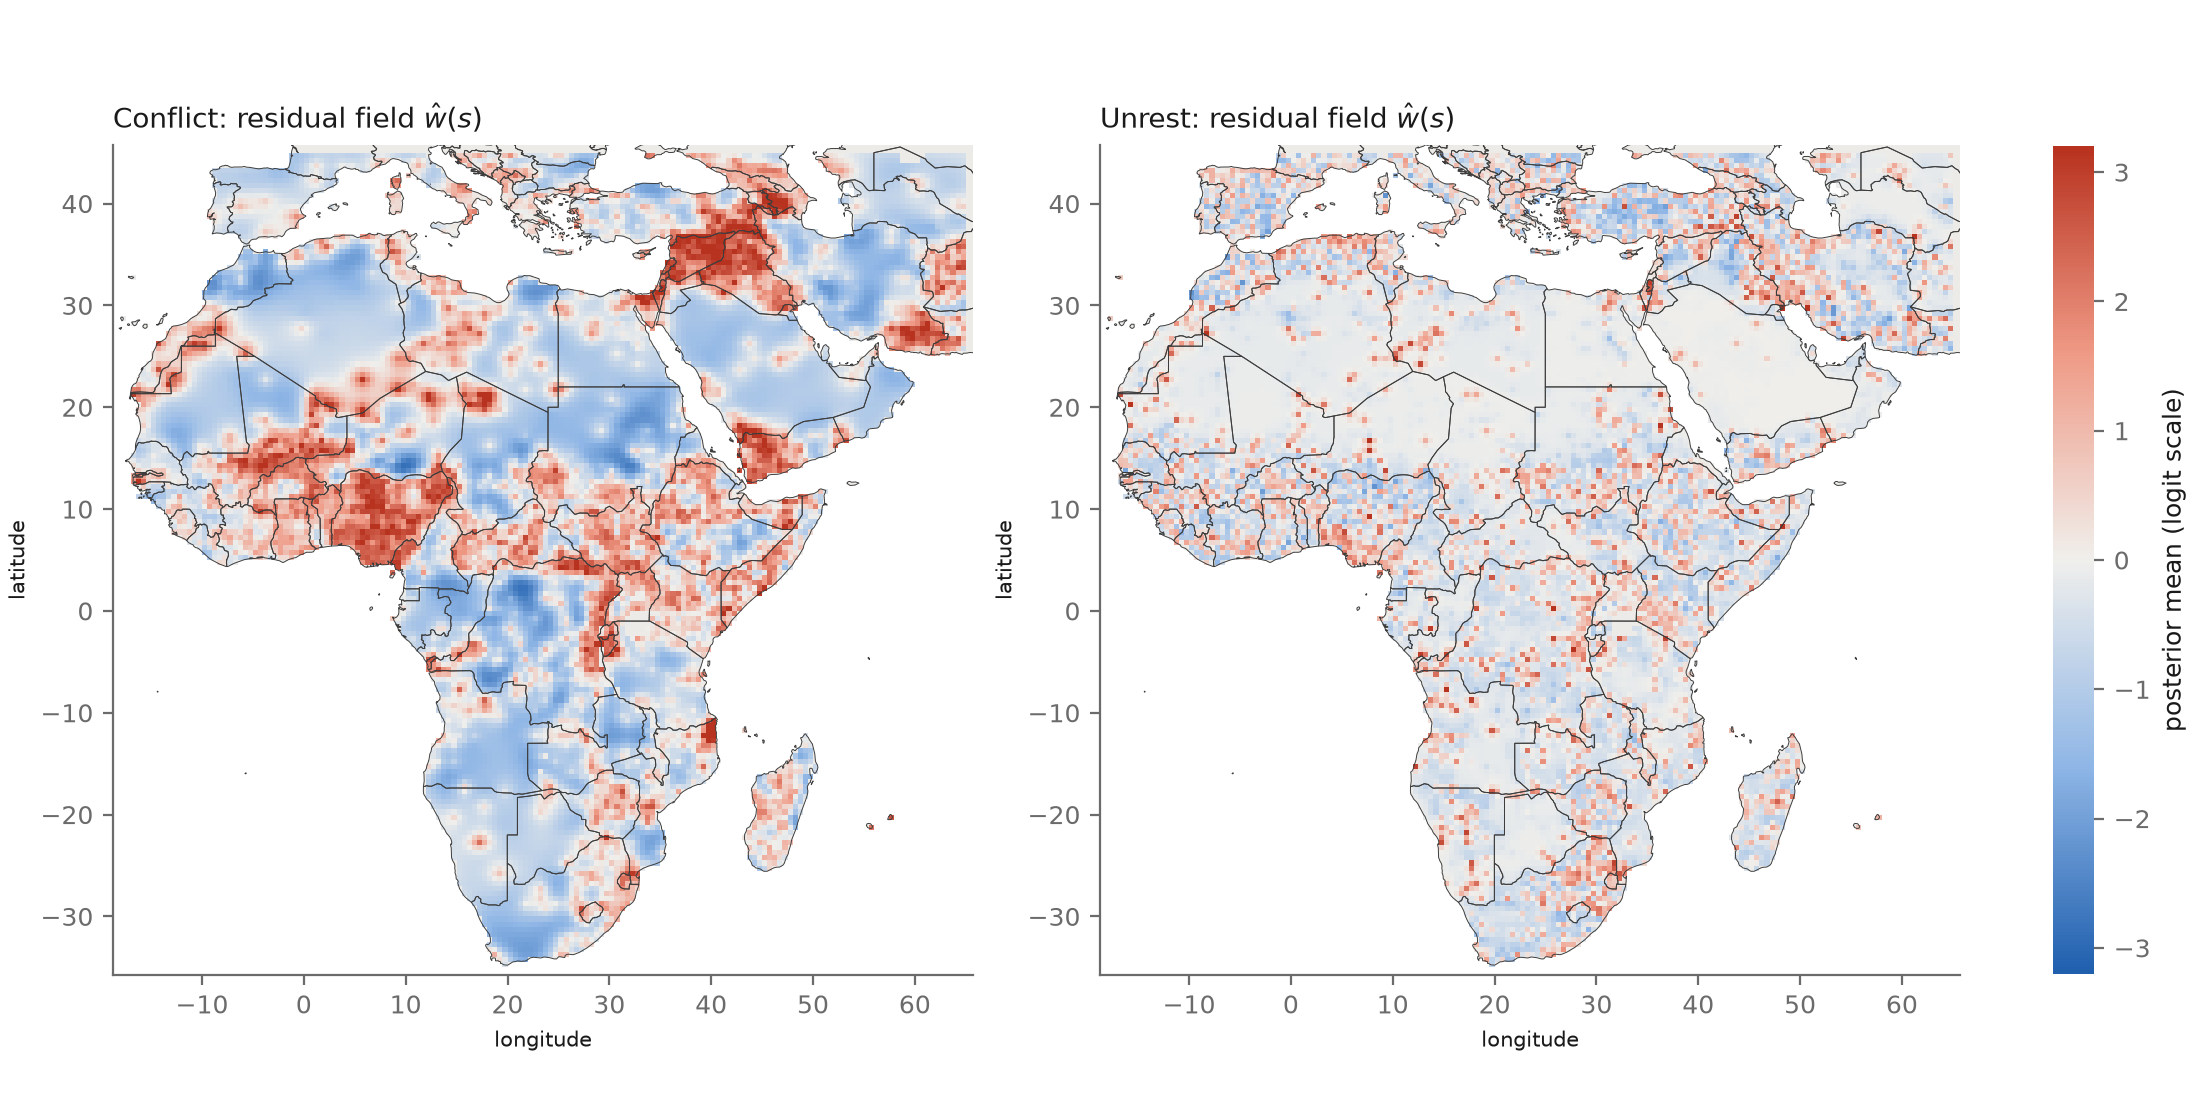
\includegraphics[width=\textwidth]{figures/real_field.png}
\caption{Posterior mean of the residual field $w(s)$ of the hybrid model for conflict
(left) and unrest (right), on the logit scale. Positive values mark persistently higher
risk than predicted by the covariates, recent event history and country
effects.}\label{fig:app-field}
\end{figure}

\begin{figure}
\centering
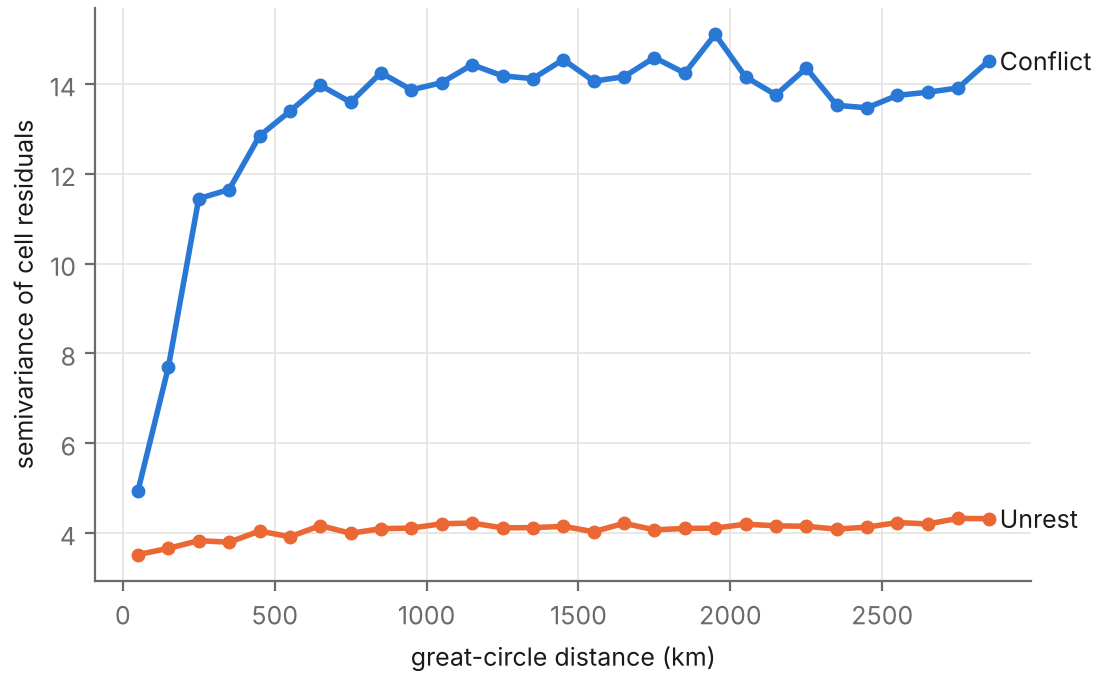
\includegraphics[width=0.6\textwidth]{figures/real_variogram.png}
\caption{Empirical semivariograms of the standardised cell residuals of the spatially
cross-fitted XGBoost model, against great-circle distance.}\label{fig:app-variogram}
\end{figure}

\subsection{State dependence, climate and national indicators}\label{sec:app-glmm}

\todo{Results of the parametric models (CRC Task 8):
(i) the state-dependence coefficient $\delta$ with lags only, with $u + w$, and with the
space-time field $v$ (Sahel and Horn of Africa);
(ii) biome means and within-biome variation of the temperature effect from the SVC model;
(iii) national indicators (EPI, footprints, GHG, V-Dem) without latent effects, with
$u + w$, and with spatial+, interpreted in the light of the confounding results of
Section~\ref{sec:sim-confounding}.}


\section{Discussion}\label{sec:discussion}

The association between recent unrest and later conflict in the same place is one of
the most robust regularities in event data, and it is often read as escalation. We
have argued that the association has a second component, shared latent episodes that
raise both kinds of events, and that models of conflict alone cannot separate the two
even when they include their own latent space-time field. A joint model in which the
two outcomes share a space-time field can. In simulations it recovers the escalation
coefficient where univariate models report escalation that does not exist, and in
ACLED data for West Africa and the Sahel and for Africa and the Middle East it
attributes between a quarter and two thirds of the univariate association to shared
episodes. Once both shared and unrest-specific episodes are modelled, a short-run
effect of recent unrest on conflict remains, of about two thirds of the univariate
estimate. \todo{Update with the Africa and Middle East refit without Europe (job 29).}

\paragraph{What the shared field represents.} The shared field is a latent component
of \emph{recorded} risk. It combines common shocks to the occurrence of conflict and
unrest, such as a political crisis, with common shocks to their reporting, such as a
period of media attention or a change in the sources that cover a region
\citep{weidmann2016closer, hellmeier2018spotlight, croicu2022reporting}. With a single
source of event data the two cannot be separated, and we do not interpret the field,
or its loading, as a property of occurrence alone. Several independent sources of
event data, or auxiliary measures of reporting intensity, would allow the two to be
distinguished \citep{cook2017twowrongs}. The same applies to the escalation
coefficient: it is a conditional association of recorded events, not a causal
effect.

\paragraph{The scale of escalation.} The joint model separates escalation from shared
episodes only at the resolution of the shared field. Escalation that unfolds over
several months and over hundreds of kilometres is indistinguishable from a shared
episode and is attributed to the field, while episodes that are shorter than a
time step or smaller than the lattice of the field remain in the lag coefficient. Our
estimate is therefore the short-run, local part of escalation. It is compatible with
accounts in which repression of protest leads to armed conflict over longer periods
\citep{ritter2016preventing, ryckman2020turn, chenoweth2017violent, rod2023protest},
and it indicates that four-week unrest histories in the same cell are a weak signal of
such escalation once shared episodes are modelled. It also explains why unrest
histories help forecasting models of conflict \citep{rod2025predicting}: they are
informative about the current episode, whatever its nature.

\paragraph{Prediction.} A more comprehensive model need not predict better. When both
outcomes are observed everywhere and both histories enter as covariates, the shared
field adds little that the univariate models do not already contain, and in our
simulations and data the joint model forecasts neither outcome better. Its predictive
value appears when one outcome is missing where the other is recorded: there the
shared field transfers information about the current episode from the observed
outcome to the unobserved one. Under-reporting of particular types of events is
common in event data \citep{weidmann2016closer, croicu2022reporting}, so this is a
practical use of the model, for example to flag areas where recorded protest
suggests that conflict may be going unrecorded. The gain fades in forecasts, because
the shared field decays at the rate of its autoregression and a shared static
field retained only a small part of it. The joint model also under-predicts the
co-occurrence of the two outcomes in the test period, by about 13--15\% in West
Africa even with a shared static field.

\paragraph{Limitations.} Several limits apply. The plug-in standard errors ignore the
uncertainty in the hyperparameters and, in simulations, understate the variability of
the lag coefficients by up to 20\% when a space-time field is fitted, so intervals
that only just exclude zero should be read with caution. The loading of the shared
field is constant in space, while the relation between unrest and conflict surely
differs between, say, the central Sahel and North Africa. Escalation runs in both
directions in the model, but the simulations covered one direction only, and they
did not reproduce the 13- and 26-week steps or the coarser lattice of the application.
The regions were chosen as boxes and the countries of Europe were excluded from the
larger one; results for other regions may differ. Finally, the analysis uses a
repaired version of an earlier cell-week table, whose construction we describe in the
Supplementary Material.

\paragraph{Extensions.} Natural extensions are loadings that vary in space, through a
second field in the loading or region-specific loadings; non-separable space-time
fields \citep{lindgren2024diffusion}; more outcomes, such as fatalities or different
actors, sharing several latent components; and hybrids with self-exciting models of
event data \citep{jun2024hawkes, browning2026hawkes}, in which the shared field would
act as a common stochastic background rate. The finite-volume construction on the
sphere and the case-control subsampling of non-events make such models feasible on
continental grids with millions of cell-weeks.


\begin{acks}[Acknowledgments]
\textit{Use of generative AI.} This work is AI-assisted. The research questions, the
choice of models and of simulation designs, the interpretation of the results and all
decisions about the analysis were made by the authors. Claude, a large language model
developed by Anthropic, accessed through the Claude Code tool between October and
November 2026, was used as an assistant under the authors' direction: (i) to write and
test computer code, including the latent Gaussian model and its Laplace-approximation
inference engine, the simulator and the simulation studies, the reconstruction of the
cell-week data set, the reproduction of the earlier boosting analysis, and the scripts
that produce the tables and figures; (ii) to help check the earlier data-processing
pipeline, which led to the errors reported in Section~\ref{sec:application}; (iii) to
help draft and edit the text and compile the bibliography; and (iv) to carry out
internal reviews of the draft before submission. The authors checked the code, results,
text and references and take full responsibility for the content of the paper. Claude is
not an author of this work. All code is available in the supplementary material.
\end{acks}

\begin{funding}
\todo{Funding.}
\end{funding}

\begin{supplement}
\stitle{Code}
\sdescription{Python implementation of the latent Gaussian model, the simulator
and all simulation studies.}
\end{supplement}

\IfFileExists{spr-ims-nameyear.bst}{\bibliographystyle{spr-ims-nameyear}}{\bibliographystyle{plainnat}}
\bibliography{refs}

\end{document}
